\documentclass{article}
\usepackage[UTF8]{ctex}
\usepackage{amsmath}
\usepackage{amssymb}
\usepackage{graphicx}
\usepackage{float}
\usepackage{datetime}
\usepackage{geometry}

\geometry{a4paper, top=2.54cm, bottom=2.54cm, left=3.18cm, right=3.18cm}

\author{刘思昀 SLST 2022522011}

\title{General Physics II 电感位移传感器特性研究}

\begin{document}

\date{\formatdate{1}{4}{2024}}

\maketitle

\section{RL分压法测电感}

\subsection{测量输出电压与位移的关系}
\begin{figure*}[htbp]
    \centering
    
\includegraphics[width=0.9\textwidth]{RL-1.png}
    \caption{RL分压法测电感-1}
\end{figure*}

\begin{figure*}[htbp]
   \centering
   
\includegraphics[width=0.9\textwidth]{RL-2.png}
   \caption{RL分压法测电感-2}
\end{figure*}

由于前面部分的输出电压和输入电压没有变化,故取中间点位置,即位移为$15mm$处为零点,此时的输入电压$V_i = 4.88 V$,输出电压$V_0 = 1.72 V$

\subsection{L计算}
\begin{equation*}
   L = \frac{R}{\omega}\sqrt{(\frac{V_i}{V_R})^2 - 1}
\end{equation*}

\begin{figure*}[htbp]
   \centering
   
\includegraphics[width=0.9\textwidth]{RL-3.png}
   \caption{RL分压法测电感自变量-1}
\end{figure*}

\begin{figure*}[htbp]
  \centering
  
\includegraphics[width=0.9\textwidth]{RL-4.png}
  \caption{RL分压法测电感自变量-2}
\end{figure*}

\begin{figure*}[htbp]
   \centering
   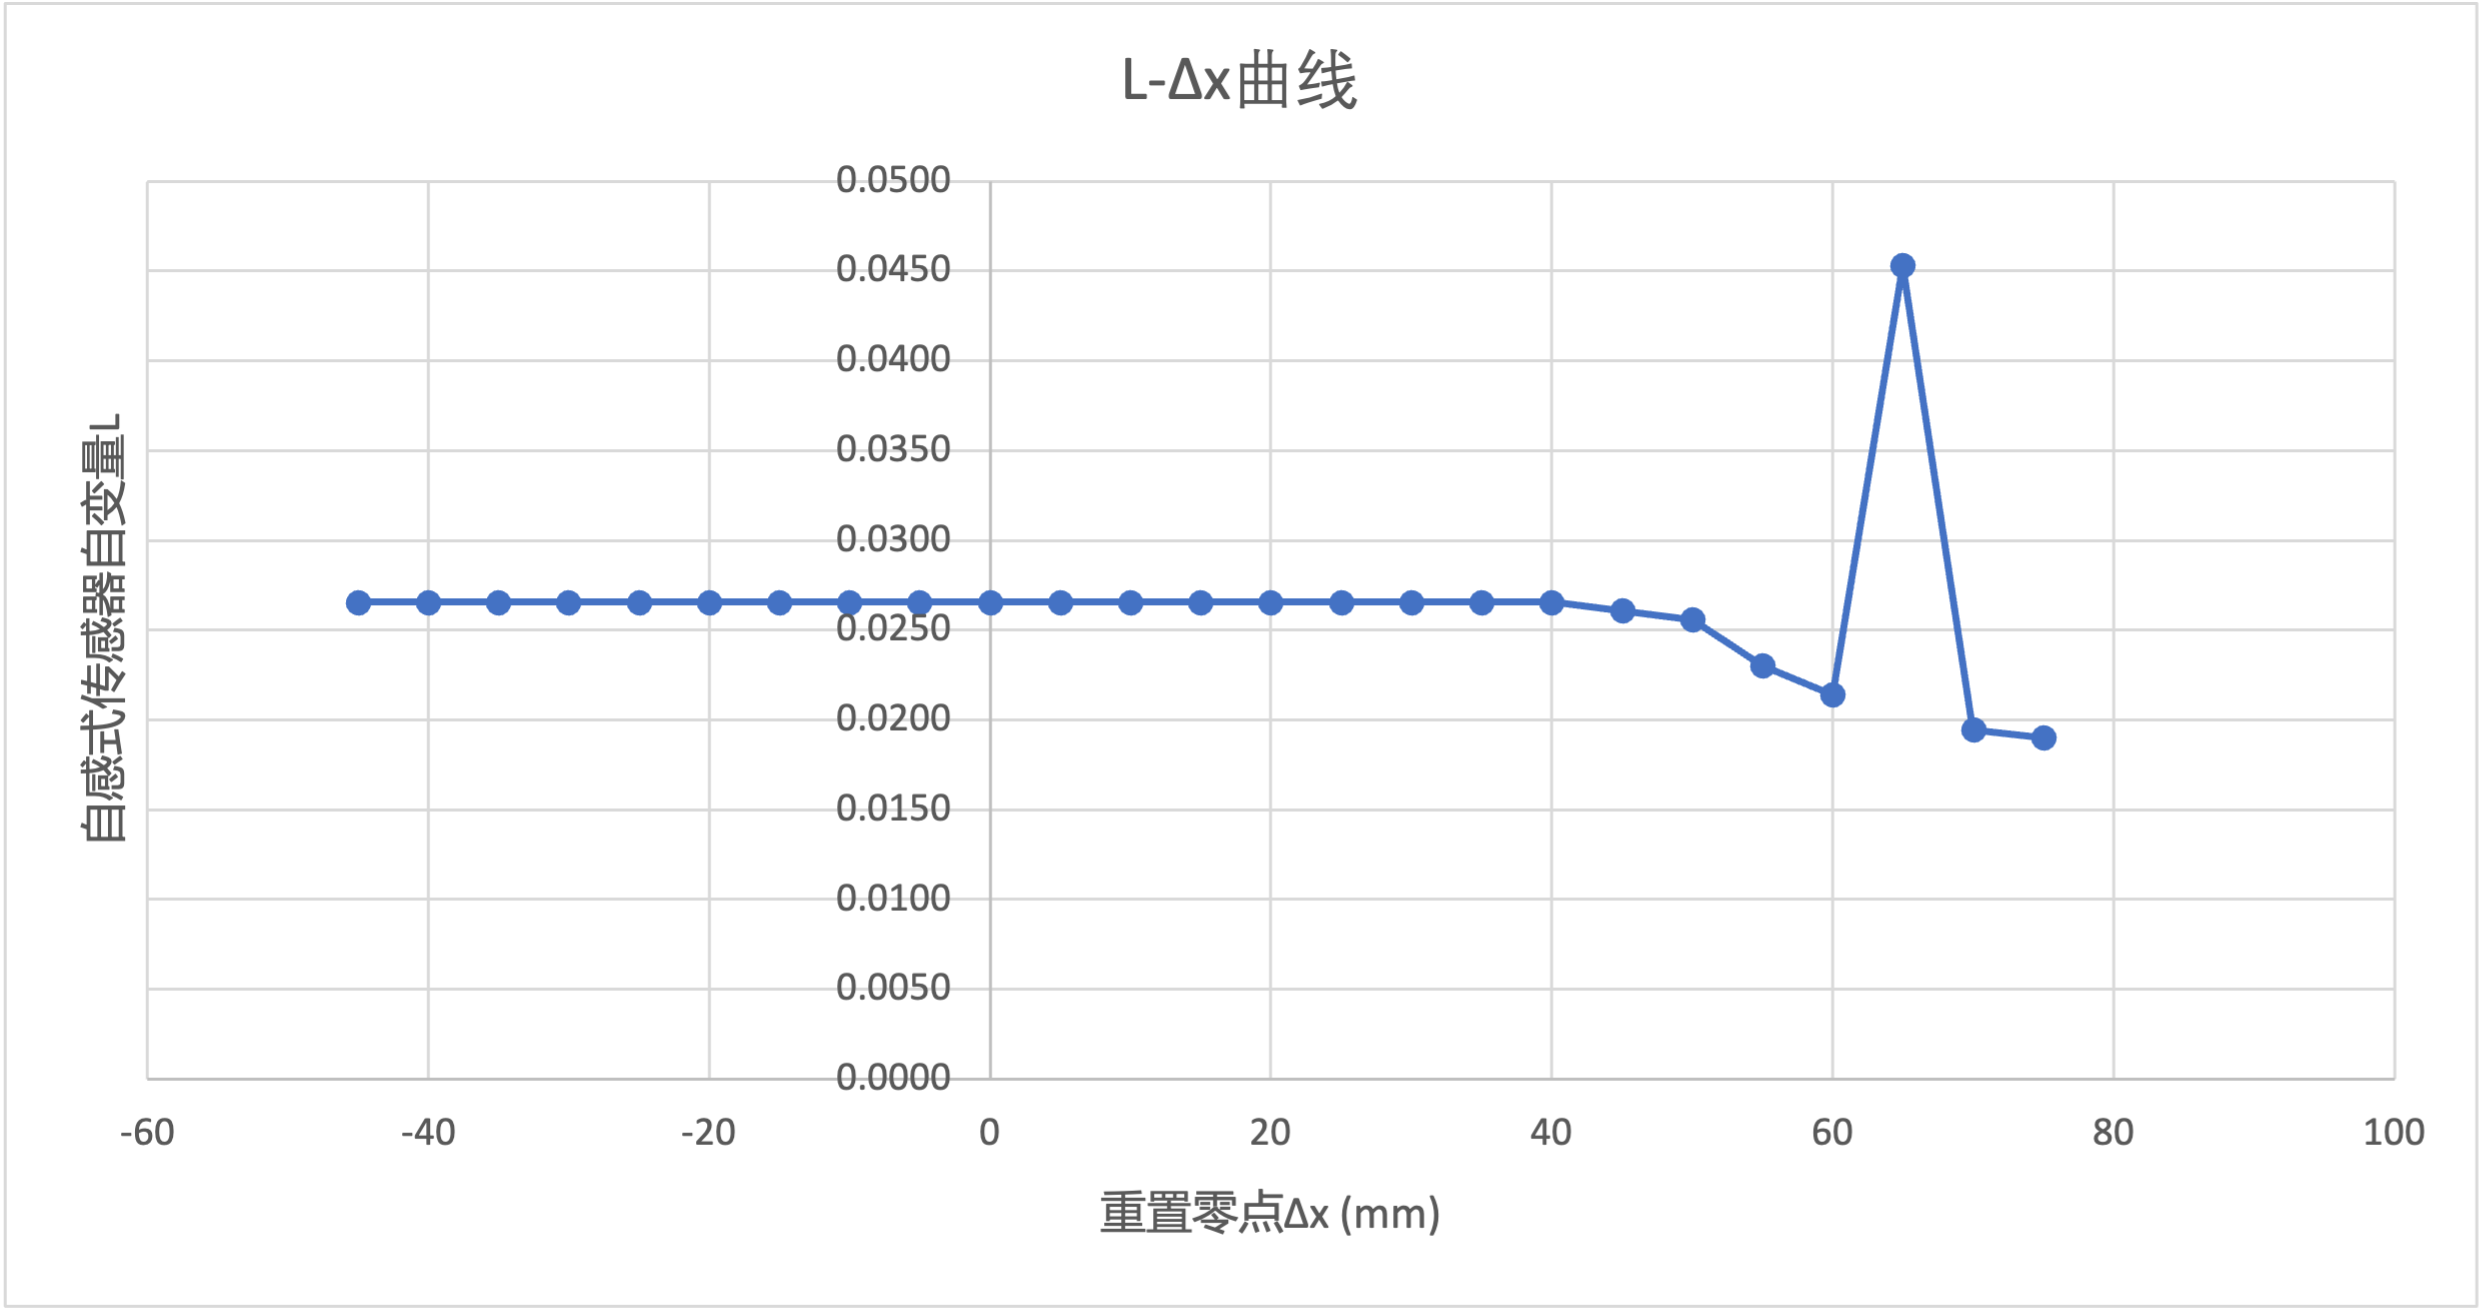
\includegraphics[width=0.7\textwidth]{RL-curve.png}
   \caption{$L-\Delta x$曲线}
 \end{figure*}

\subsection{结论}
忽略重置零点$\Delta x = 0 mm$的异常值,沿着磁棒方向,中间位置的磁通基本不变,在两端会减小。

\newpage

\section{用示波器测量差动变压器的输出}

\subsection{模仿铁芯移动工作模式}
\begin{equation*}
   U_0 = \frac{V_0}{V_{0max}}, V_{0max} = 0.880 V
\end{equation*}

\begin{figure*}[htbp]
   \centering
   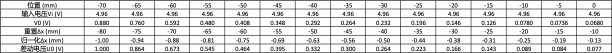
\includegraphics[width=0.9\textwidth]{osc-1.png}
   \caption{模仿铁芯移动工作模式输入电压$V_i$变化-1}
 \end{figure*}

\begin{figure*}[htbp]
   \centering
   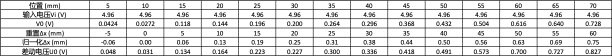
\includegraphics[width=0.9\textwidth]{osc-2.png}
   \caption{模仿铁芯移动工作模式输入电压$V_i$变化-2}
\end{figure*}

观察到在位移为$10 mm$时,差动电压$U_0$最小,将该位置极为$\Delta x$的零点。

作输出电压$U_0 - \Delta x$曲线

\begin{figure*}[htbp]
   \centering
   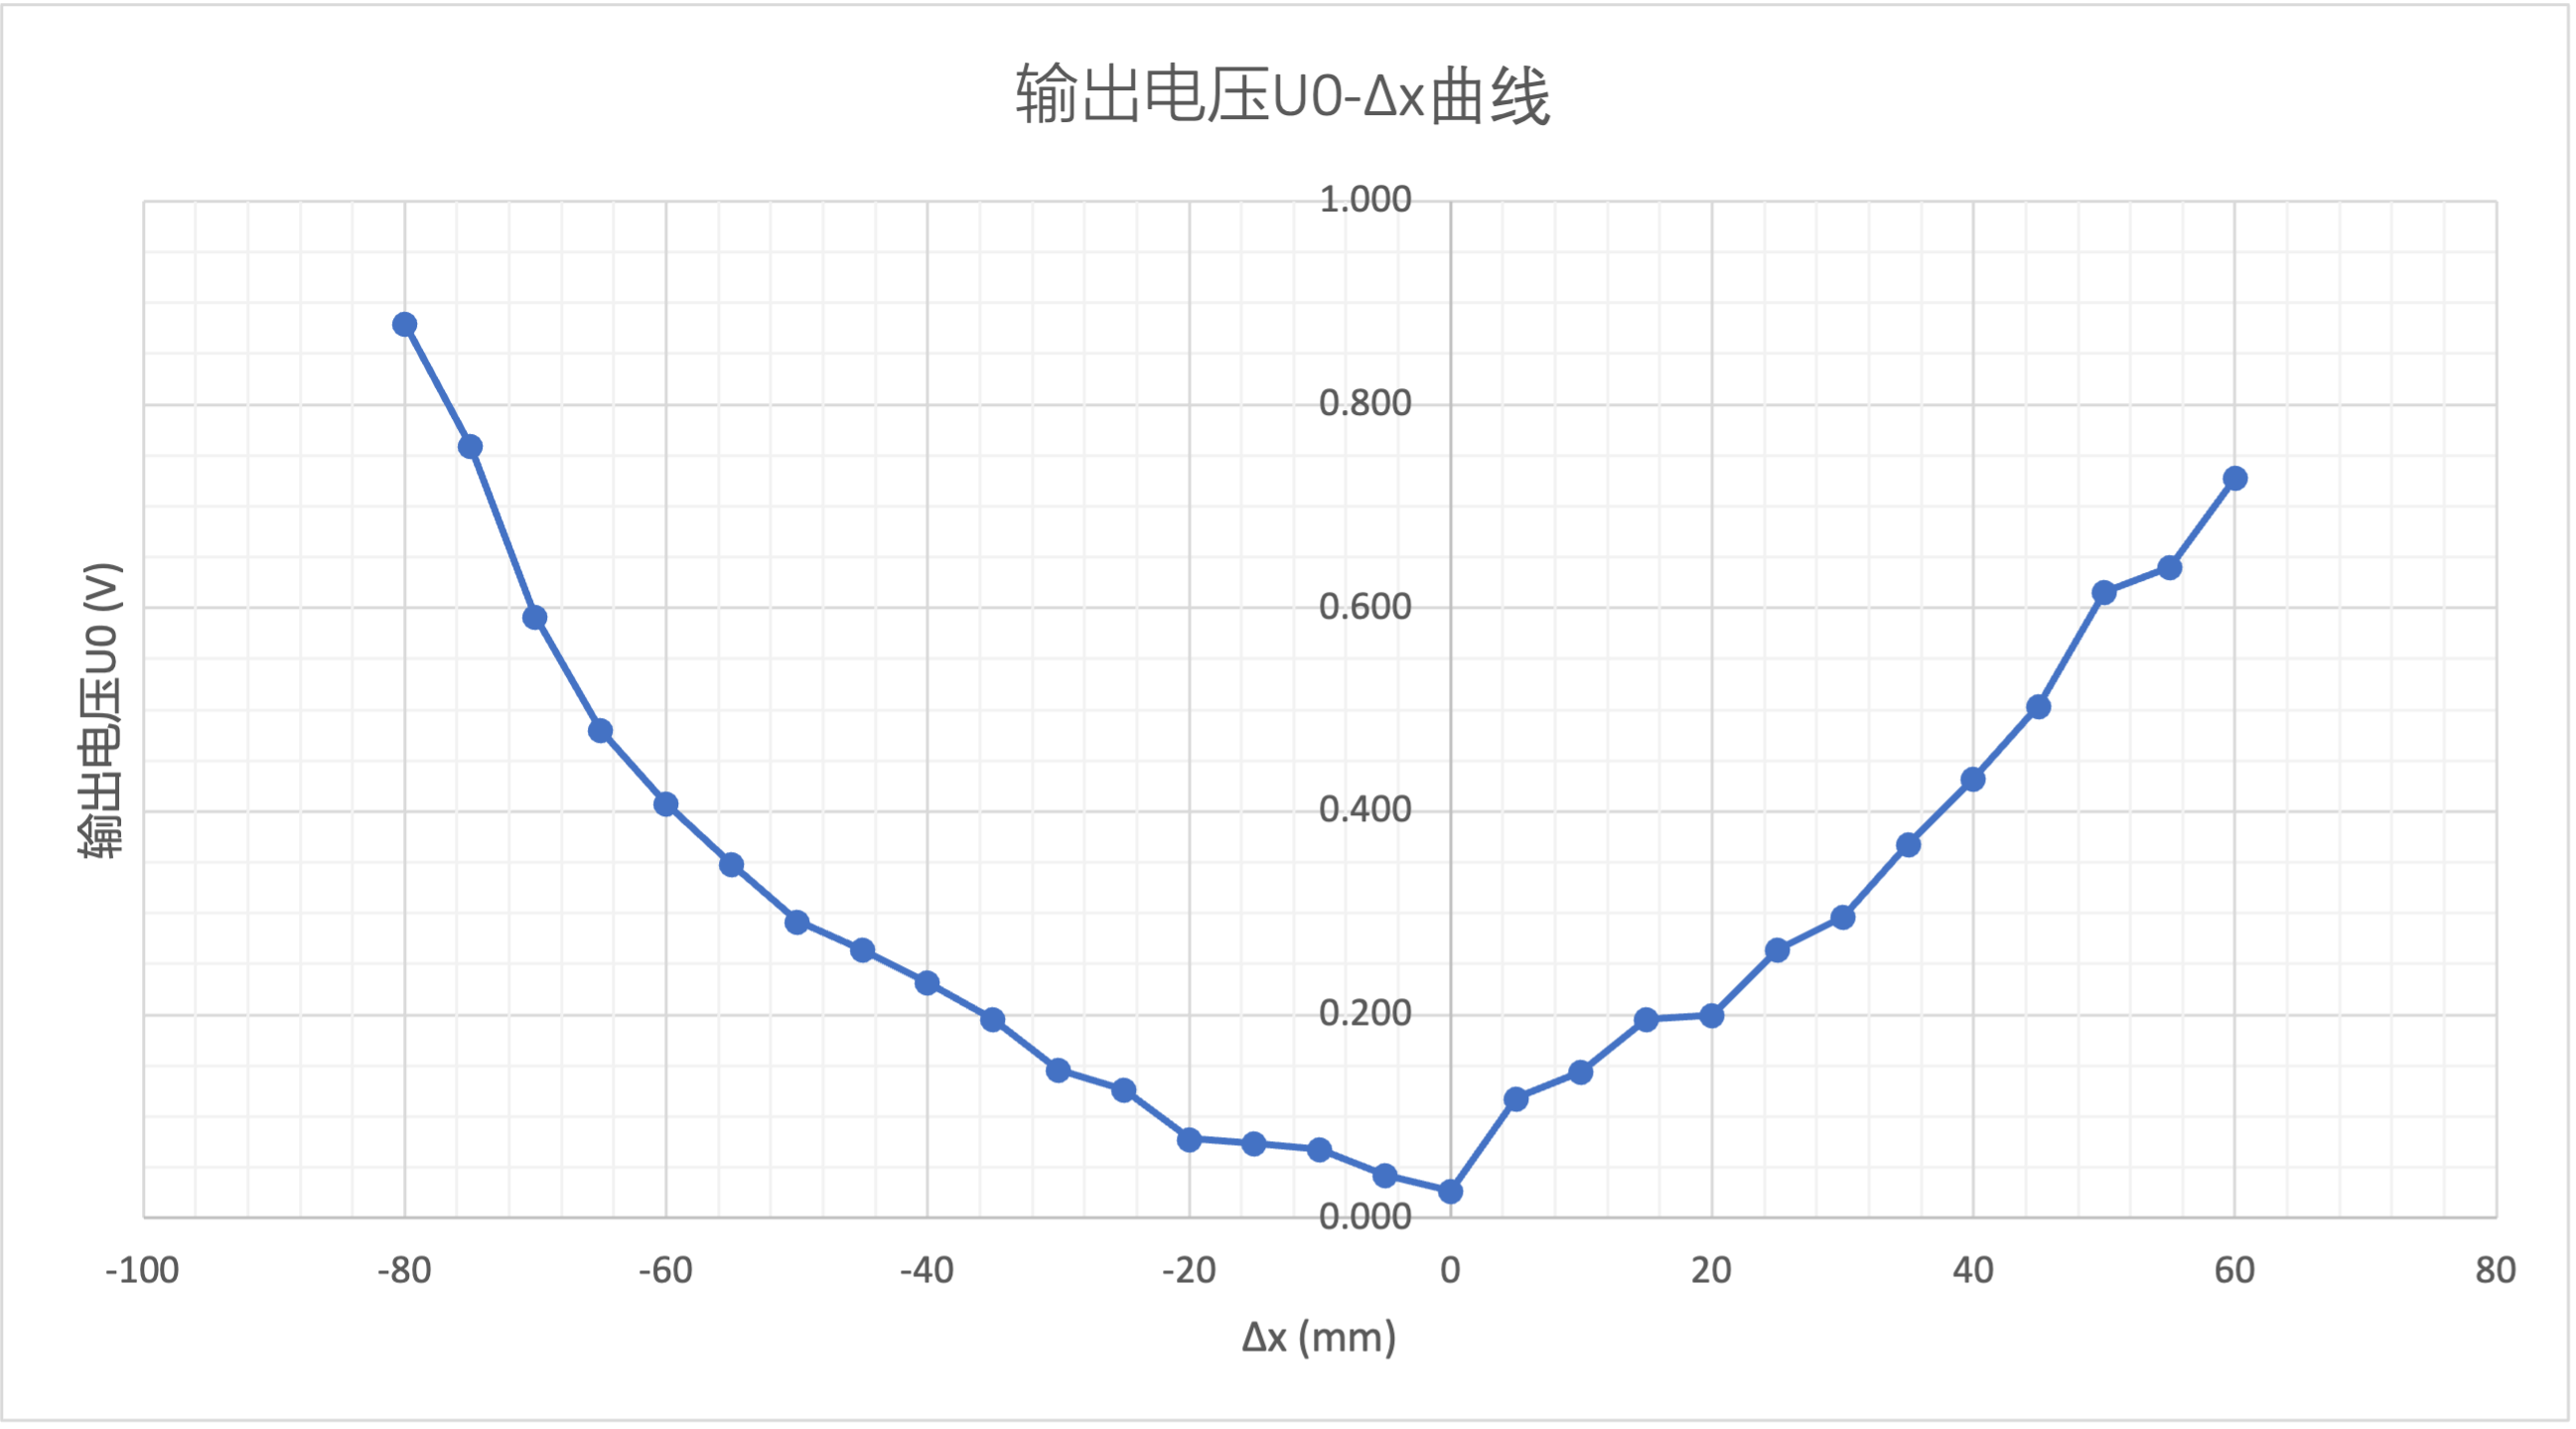
\includegraphics[width=0.7\textwidth]{osc-curve1.png}
   \caption{模仿铁芯移动工作模式输出电压$U_0 - \Delta x$曲线}
 \end{figure*}

\begin{figure*}[htbp]
   \centering
   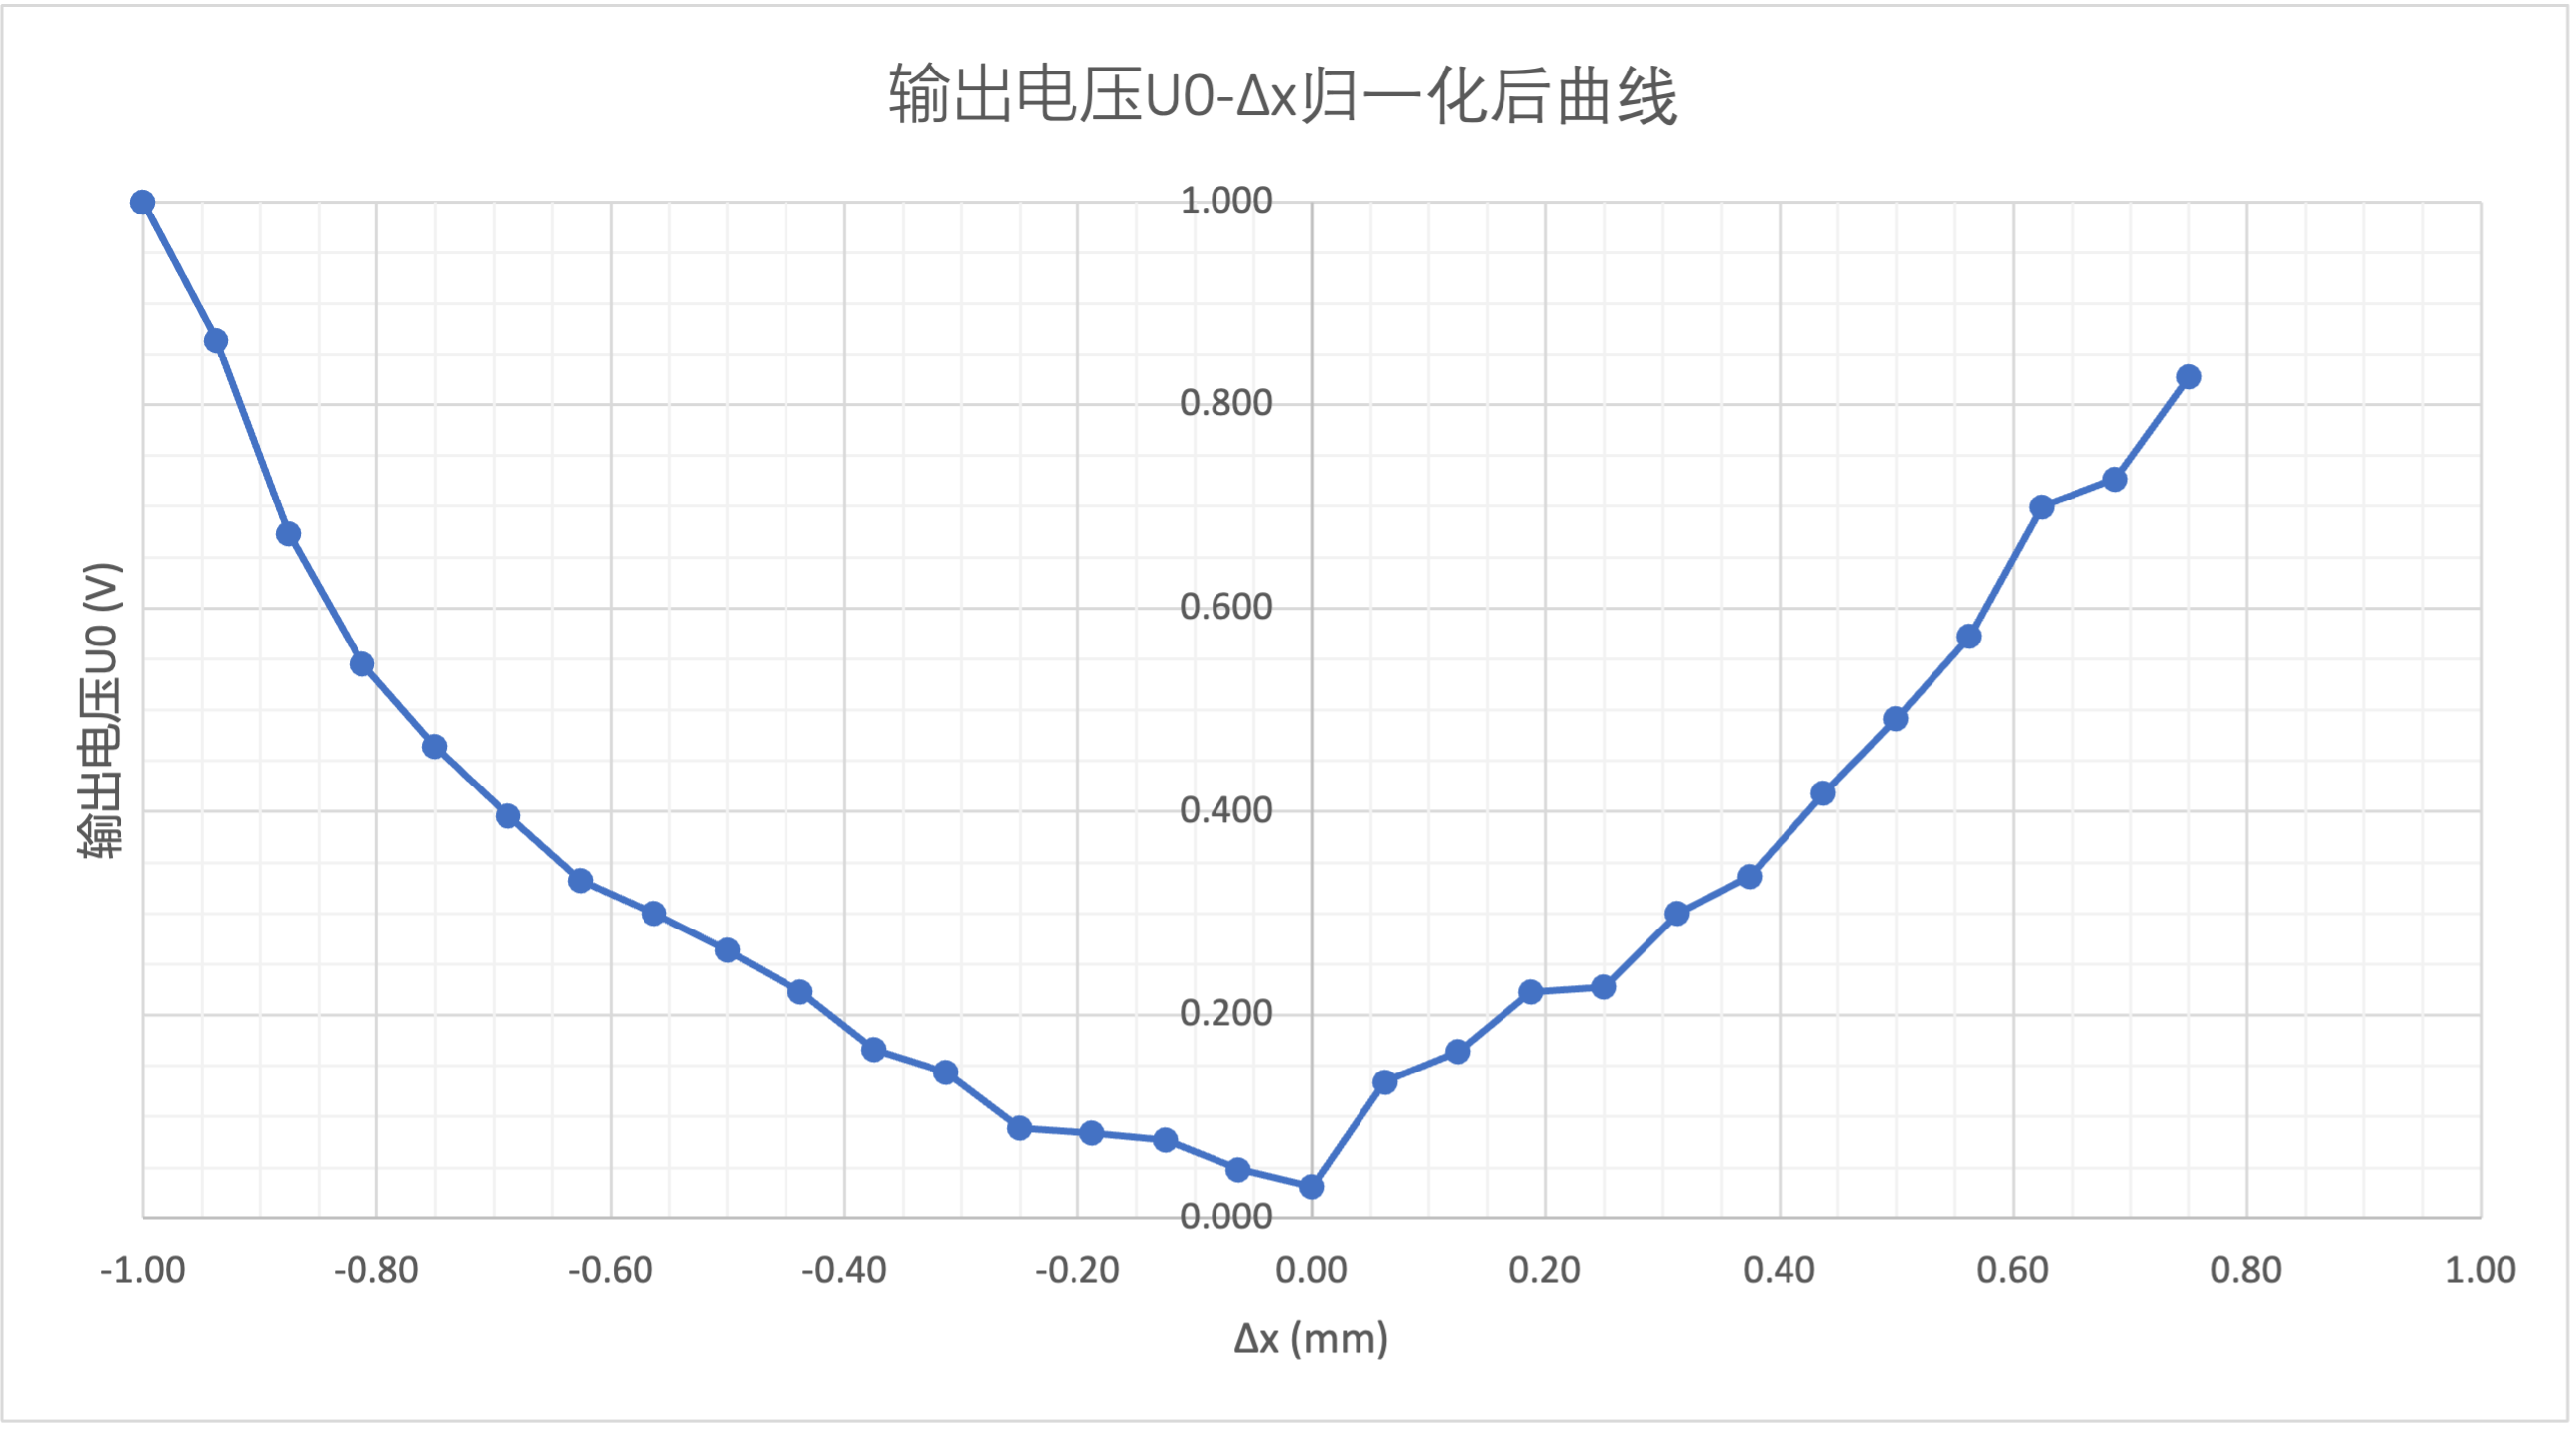
\includegraphics[width=0.7\textwidth]{osc-curve2.png}
   \caption{模仿铁芯移动工作模式输出电压$U_0 - \Delta x$归一化曲线}
\end{figure*}

\newpage

\subsection{模仿电感移动工作模式}
\begin{equation*}
   U_0 = \frac{V_0}{V_{0max}}, V_{0max} = 2.94 V
\end{equation*}

\begin{figure*}[htbp]
   \centering
   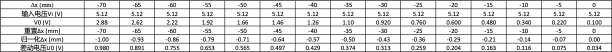
\includegraphics[width=0.9\textwidth]{osc-3.png}
   \caption{模仿电感移动工作模式输入电压$V_i$变化-1}
 \end{figure*}

\begin{figure*}[htbp]
   \centering
   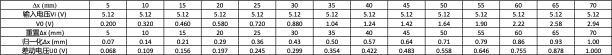
\includegraphics[width=0.9\textwidth]{osc-4.png}
   \caption{模仿电感移动工作模式输入电压$V_i$变化-2}
\end{figure*}

观察到在位移为$0 mm$时,差动电压$U_0$最小,将该位置极为$\Delta x$的零点。

作输出电压$U_0 - \Delta x$曲线

\begin{figure*}[htbp]
   \centering
   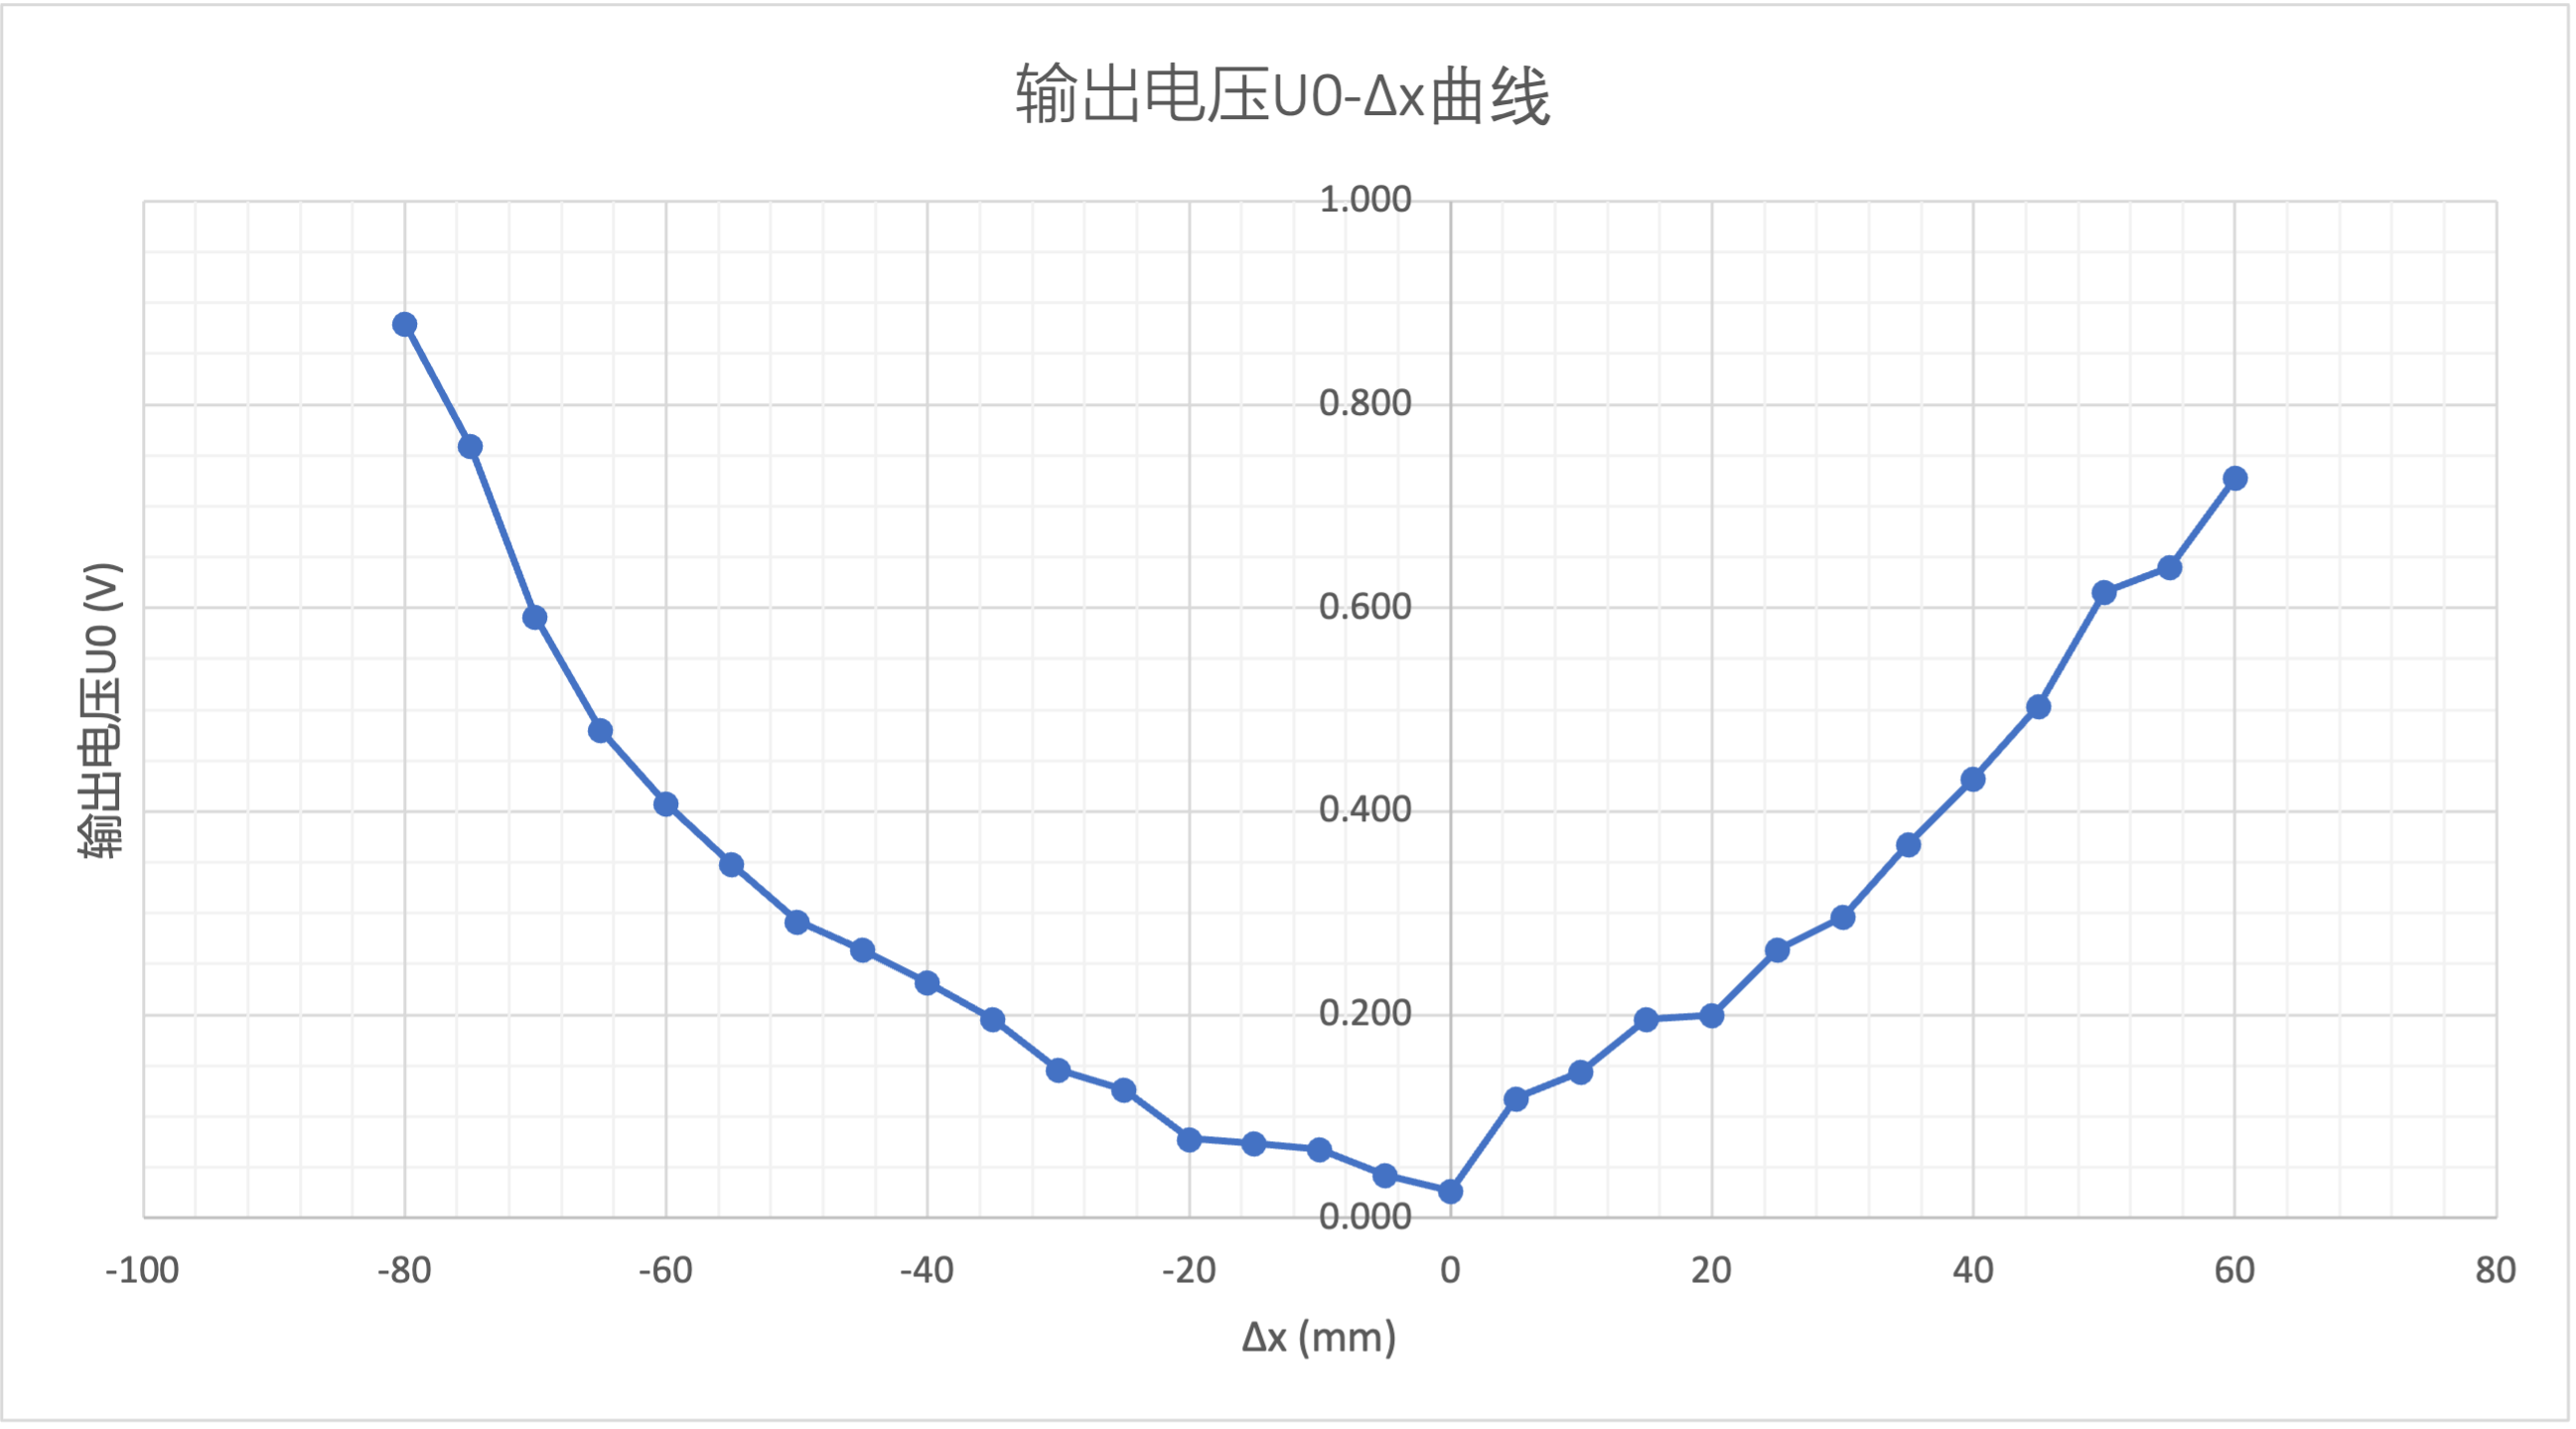
\includegraphics[width=0.7\textwidth]{osc-curve1.png}
   \caption{模仿铁芯移动工作模式输出电压$U_0 - \Delta x$曲线}
 \end{figure*}

\begin{figure*}[htbp]
   \centering
   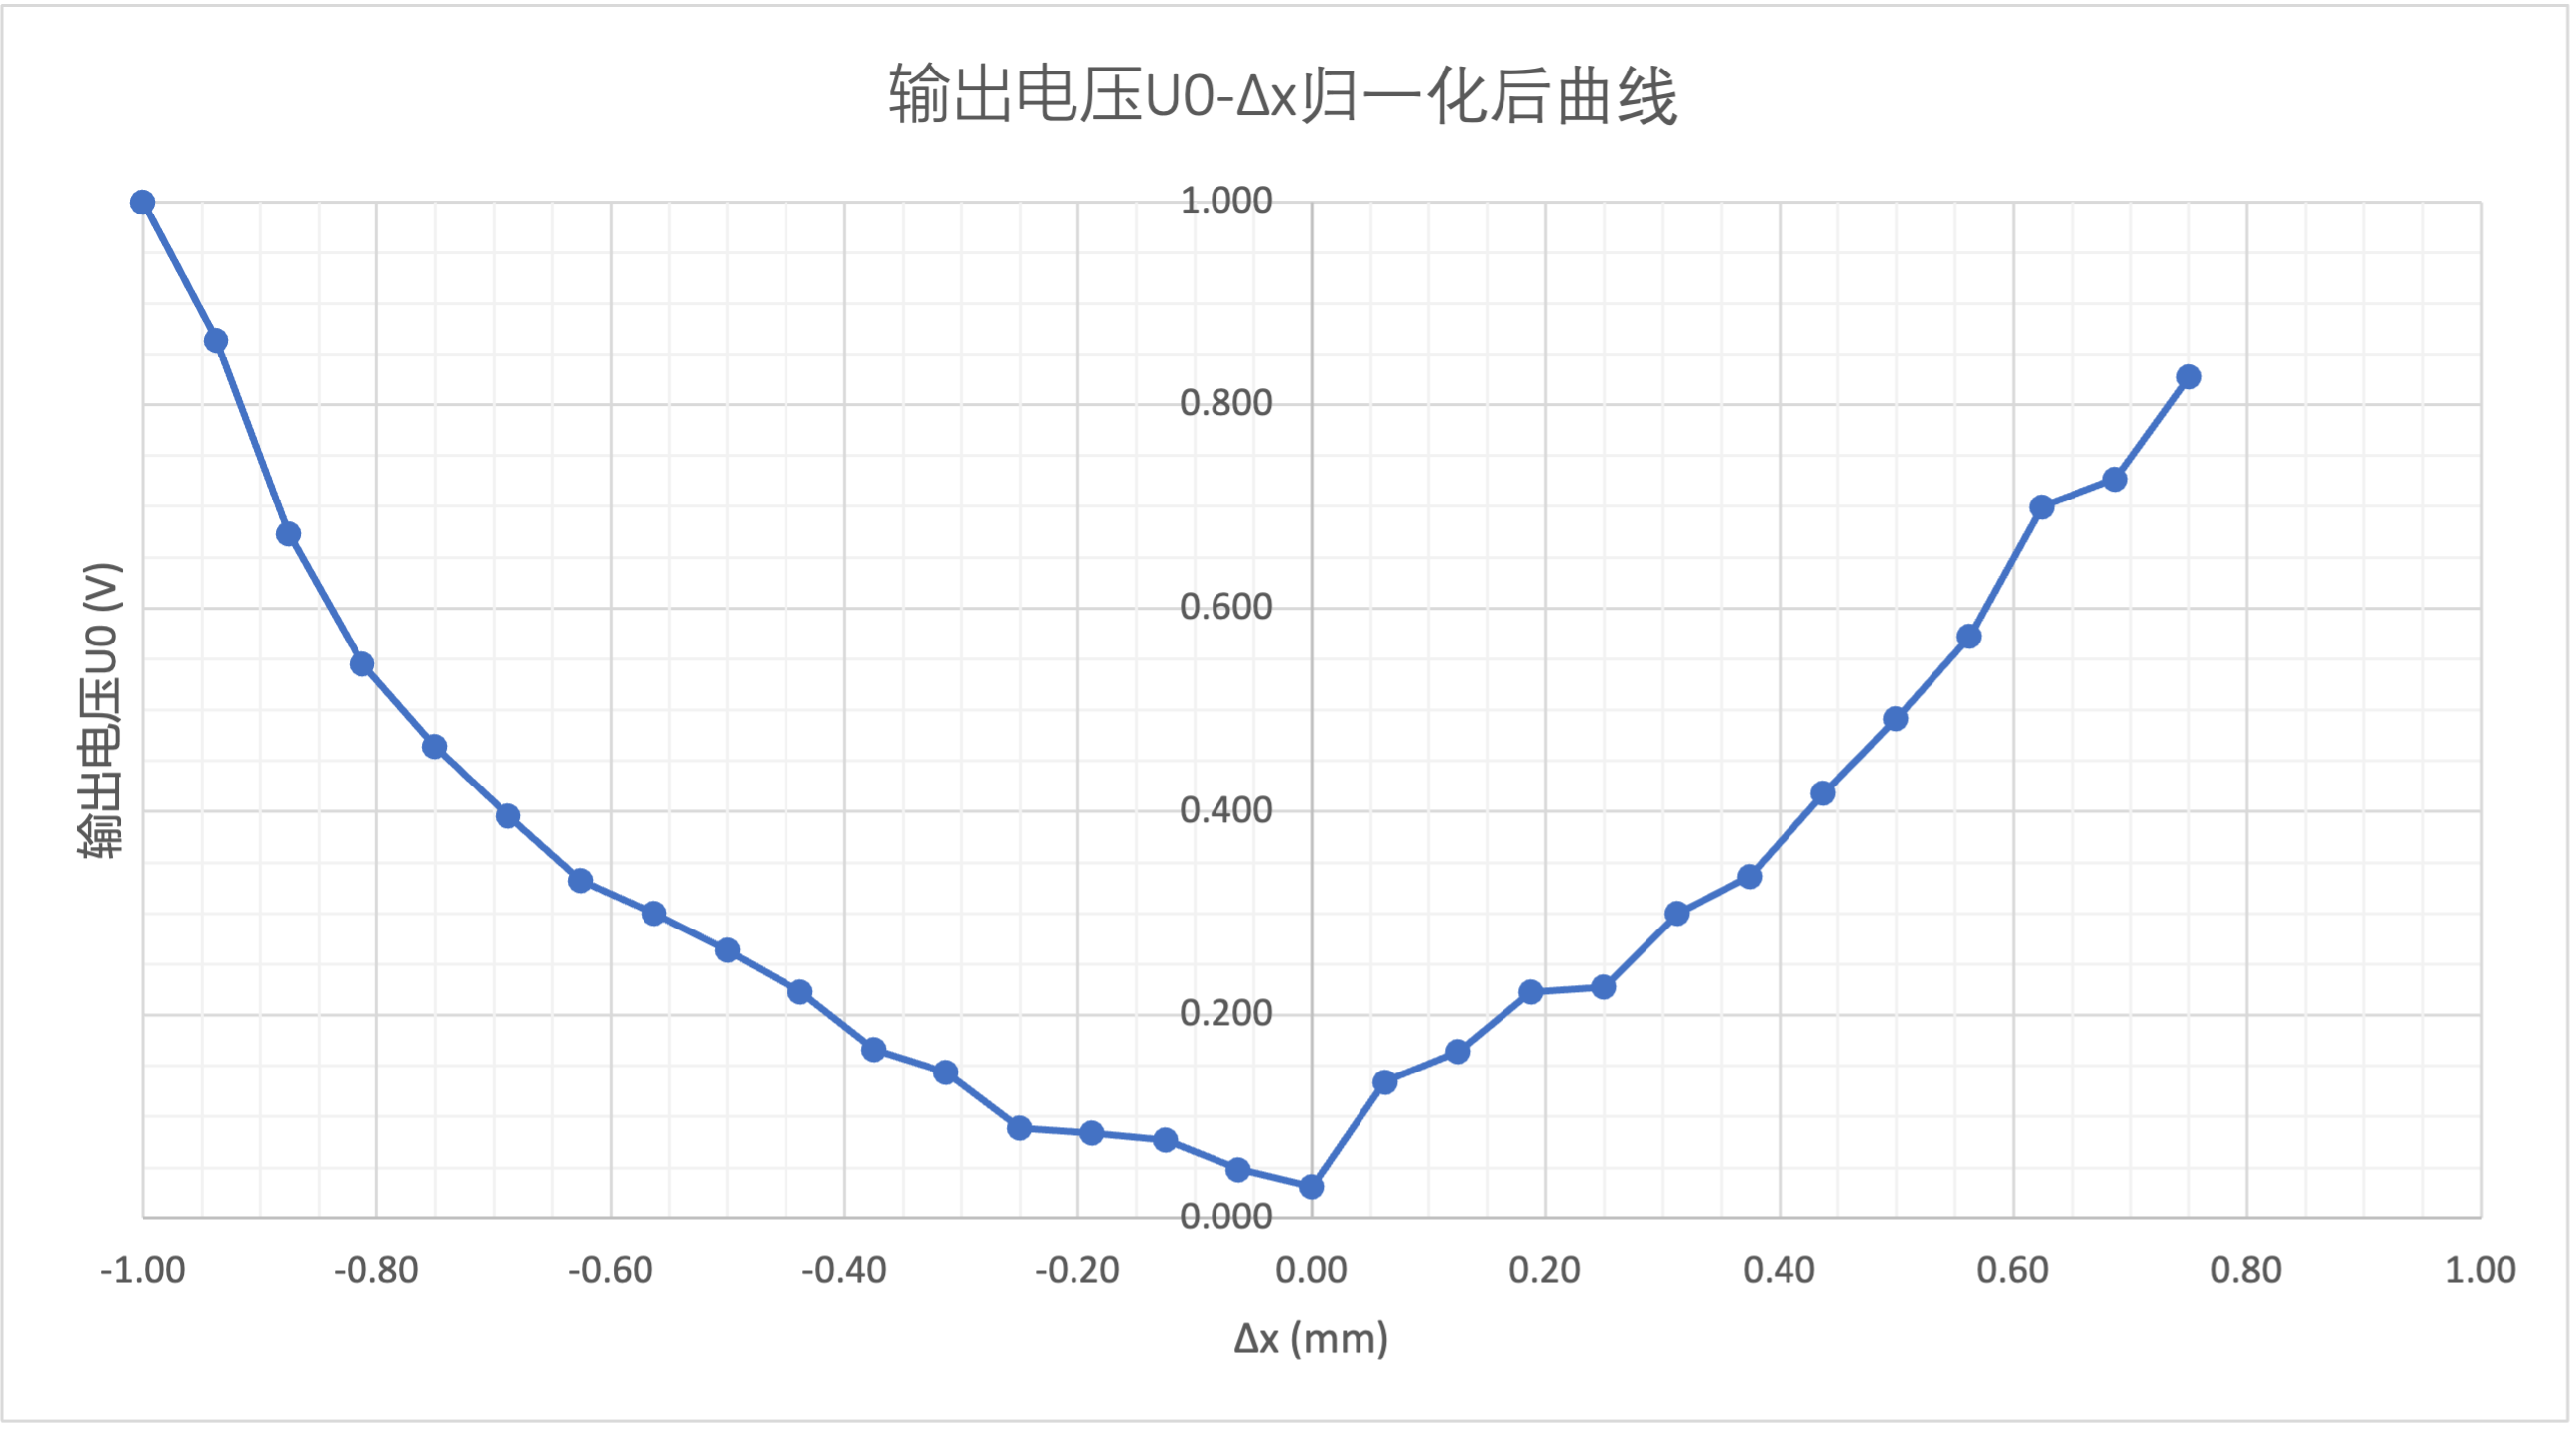
\includegraphics[width=0.7\textwidth]{osc-curve2.png}
   \caption{模仿铁芯移动工作模式输出电压$U_0 - \Delta x$归一化曲线}
\end{figure*}

\newpage

\subsection{改变激励信号频率}
\begin{figure*}[htbp]
   \centering
   
\includegraphics[width=0.6\textwidth]{osc-5.png}
   \caption{输出电压对激励信号频率的变化}
\end{figure*}

\begin{figure*}[htbp]
   \centering
   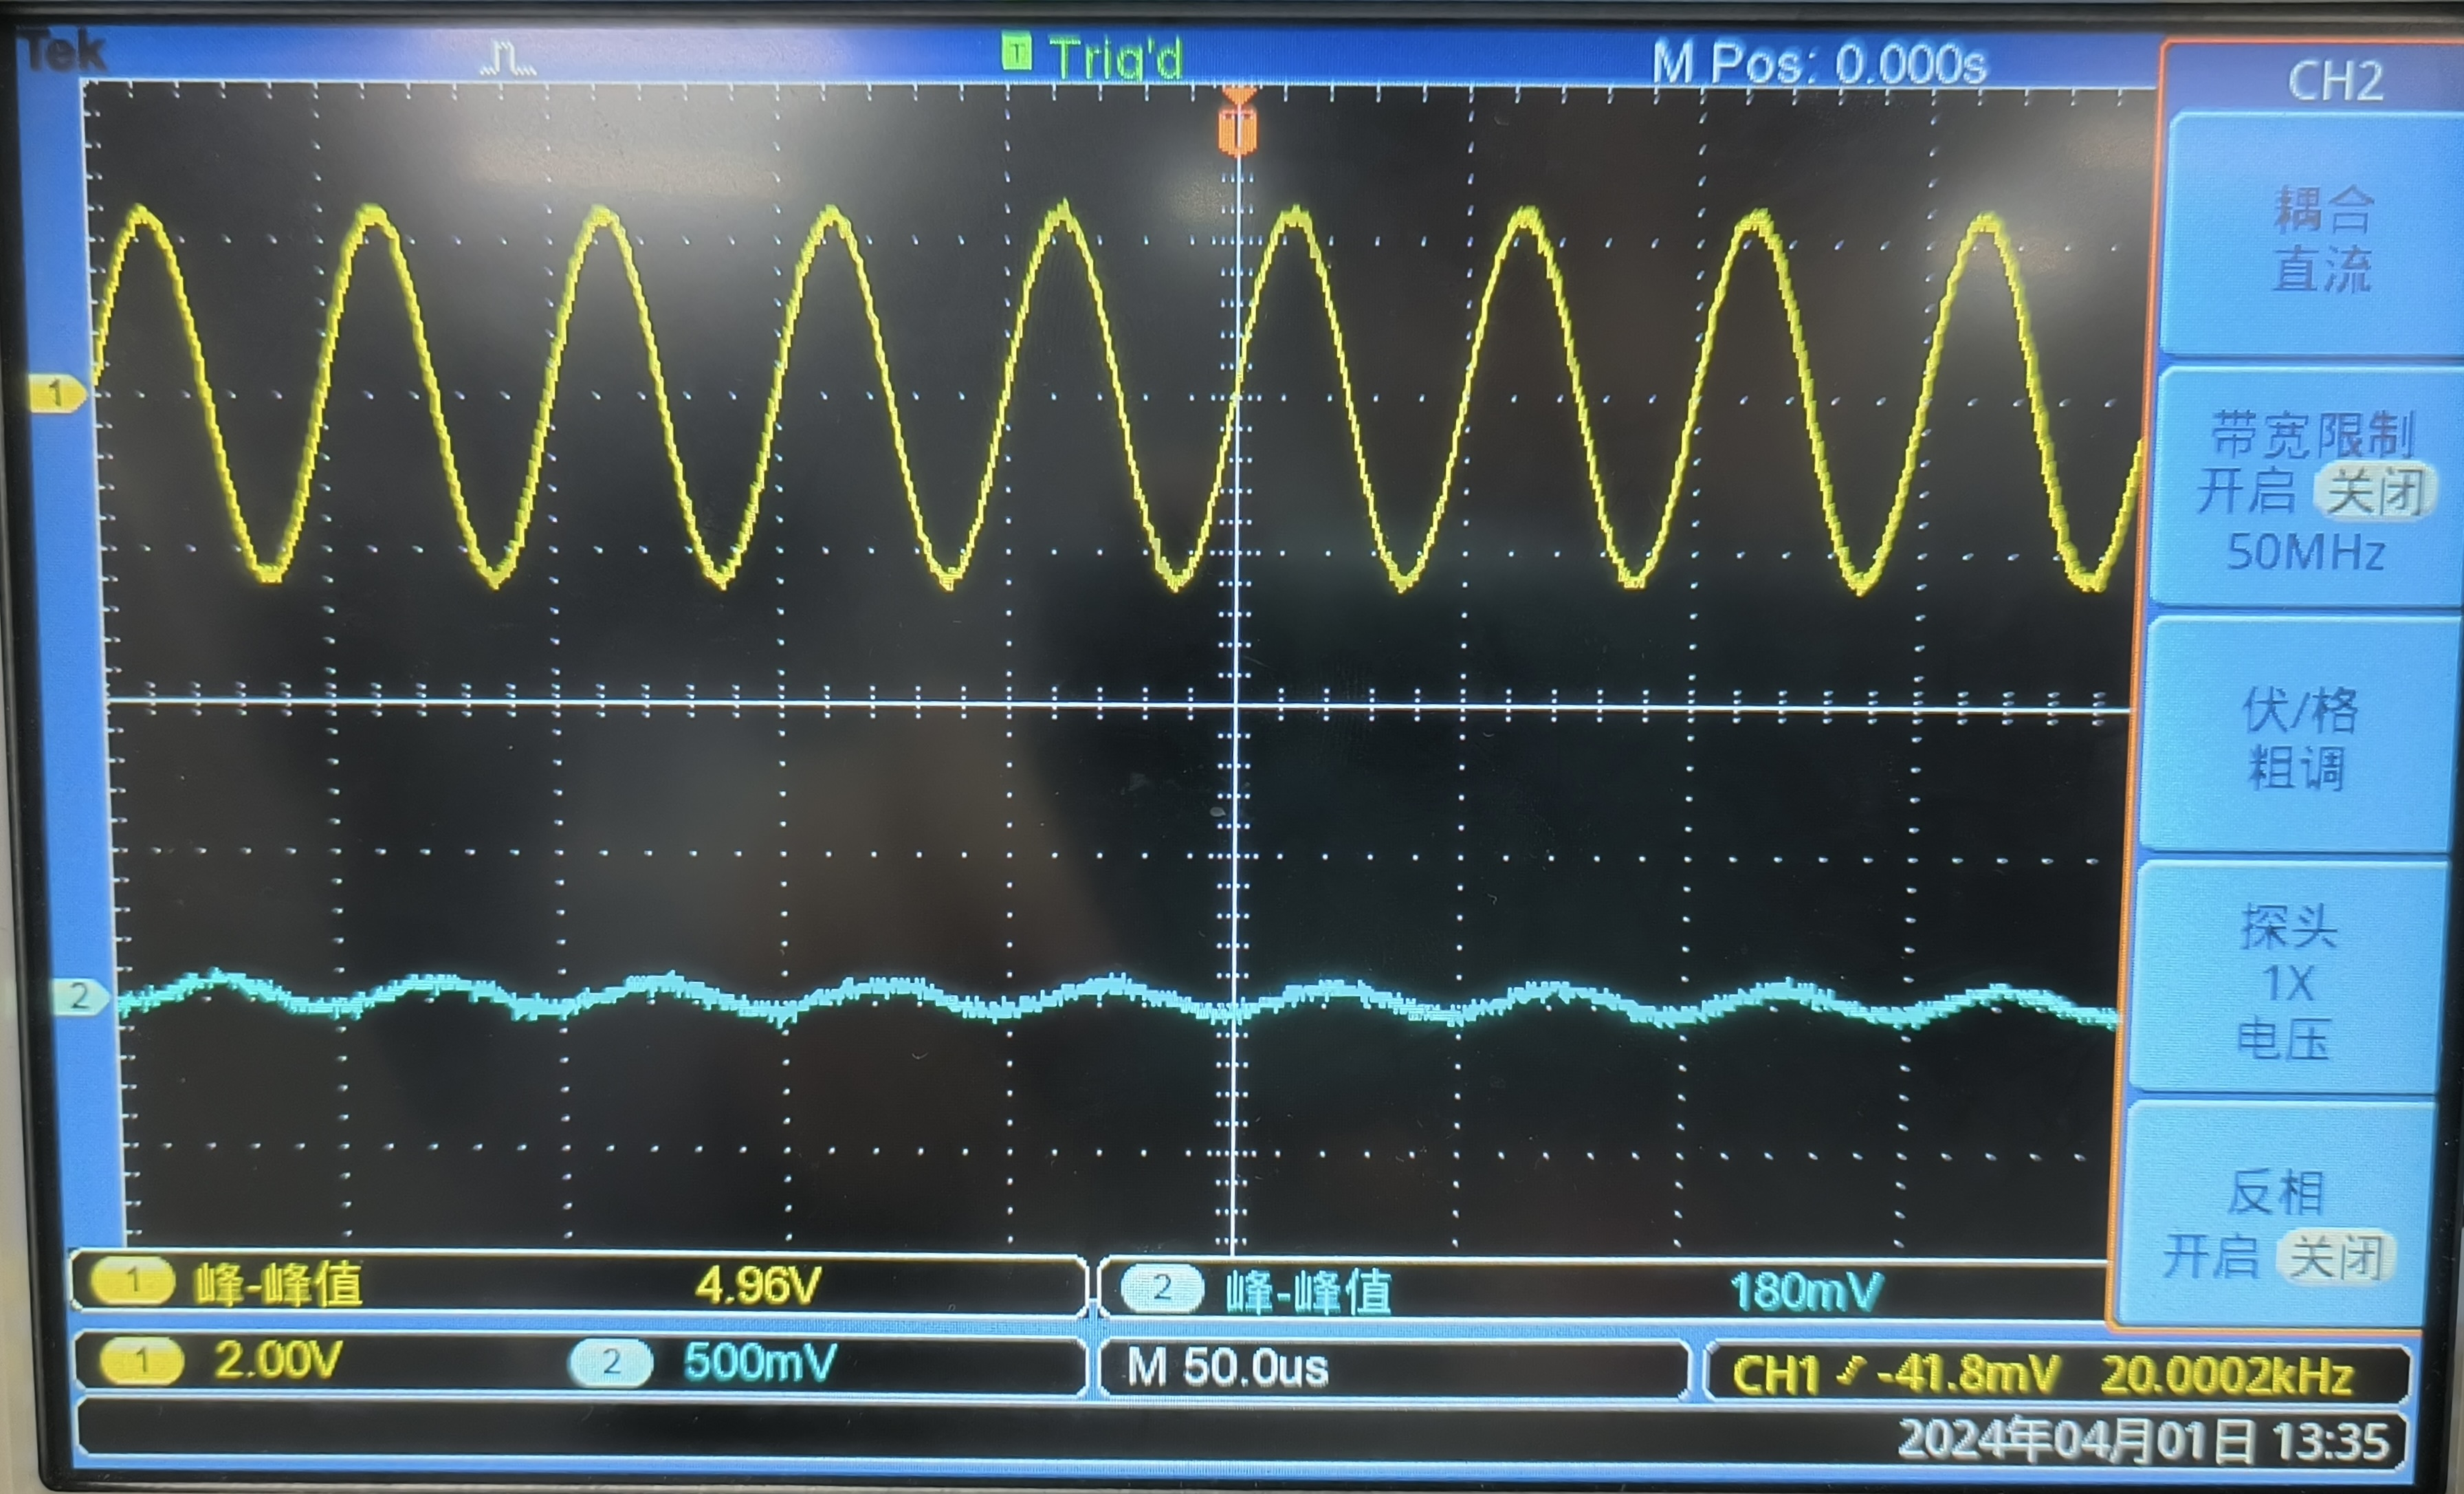
\includegraphics[width=0.6\textwidth]{20k.jpeg}
   \caption{激励信号为20kHz时波形图}
\end{figure*}

\begin{figure*}[htbp]
   \centering
   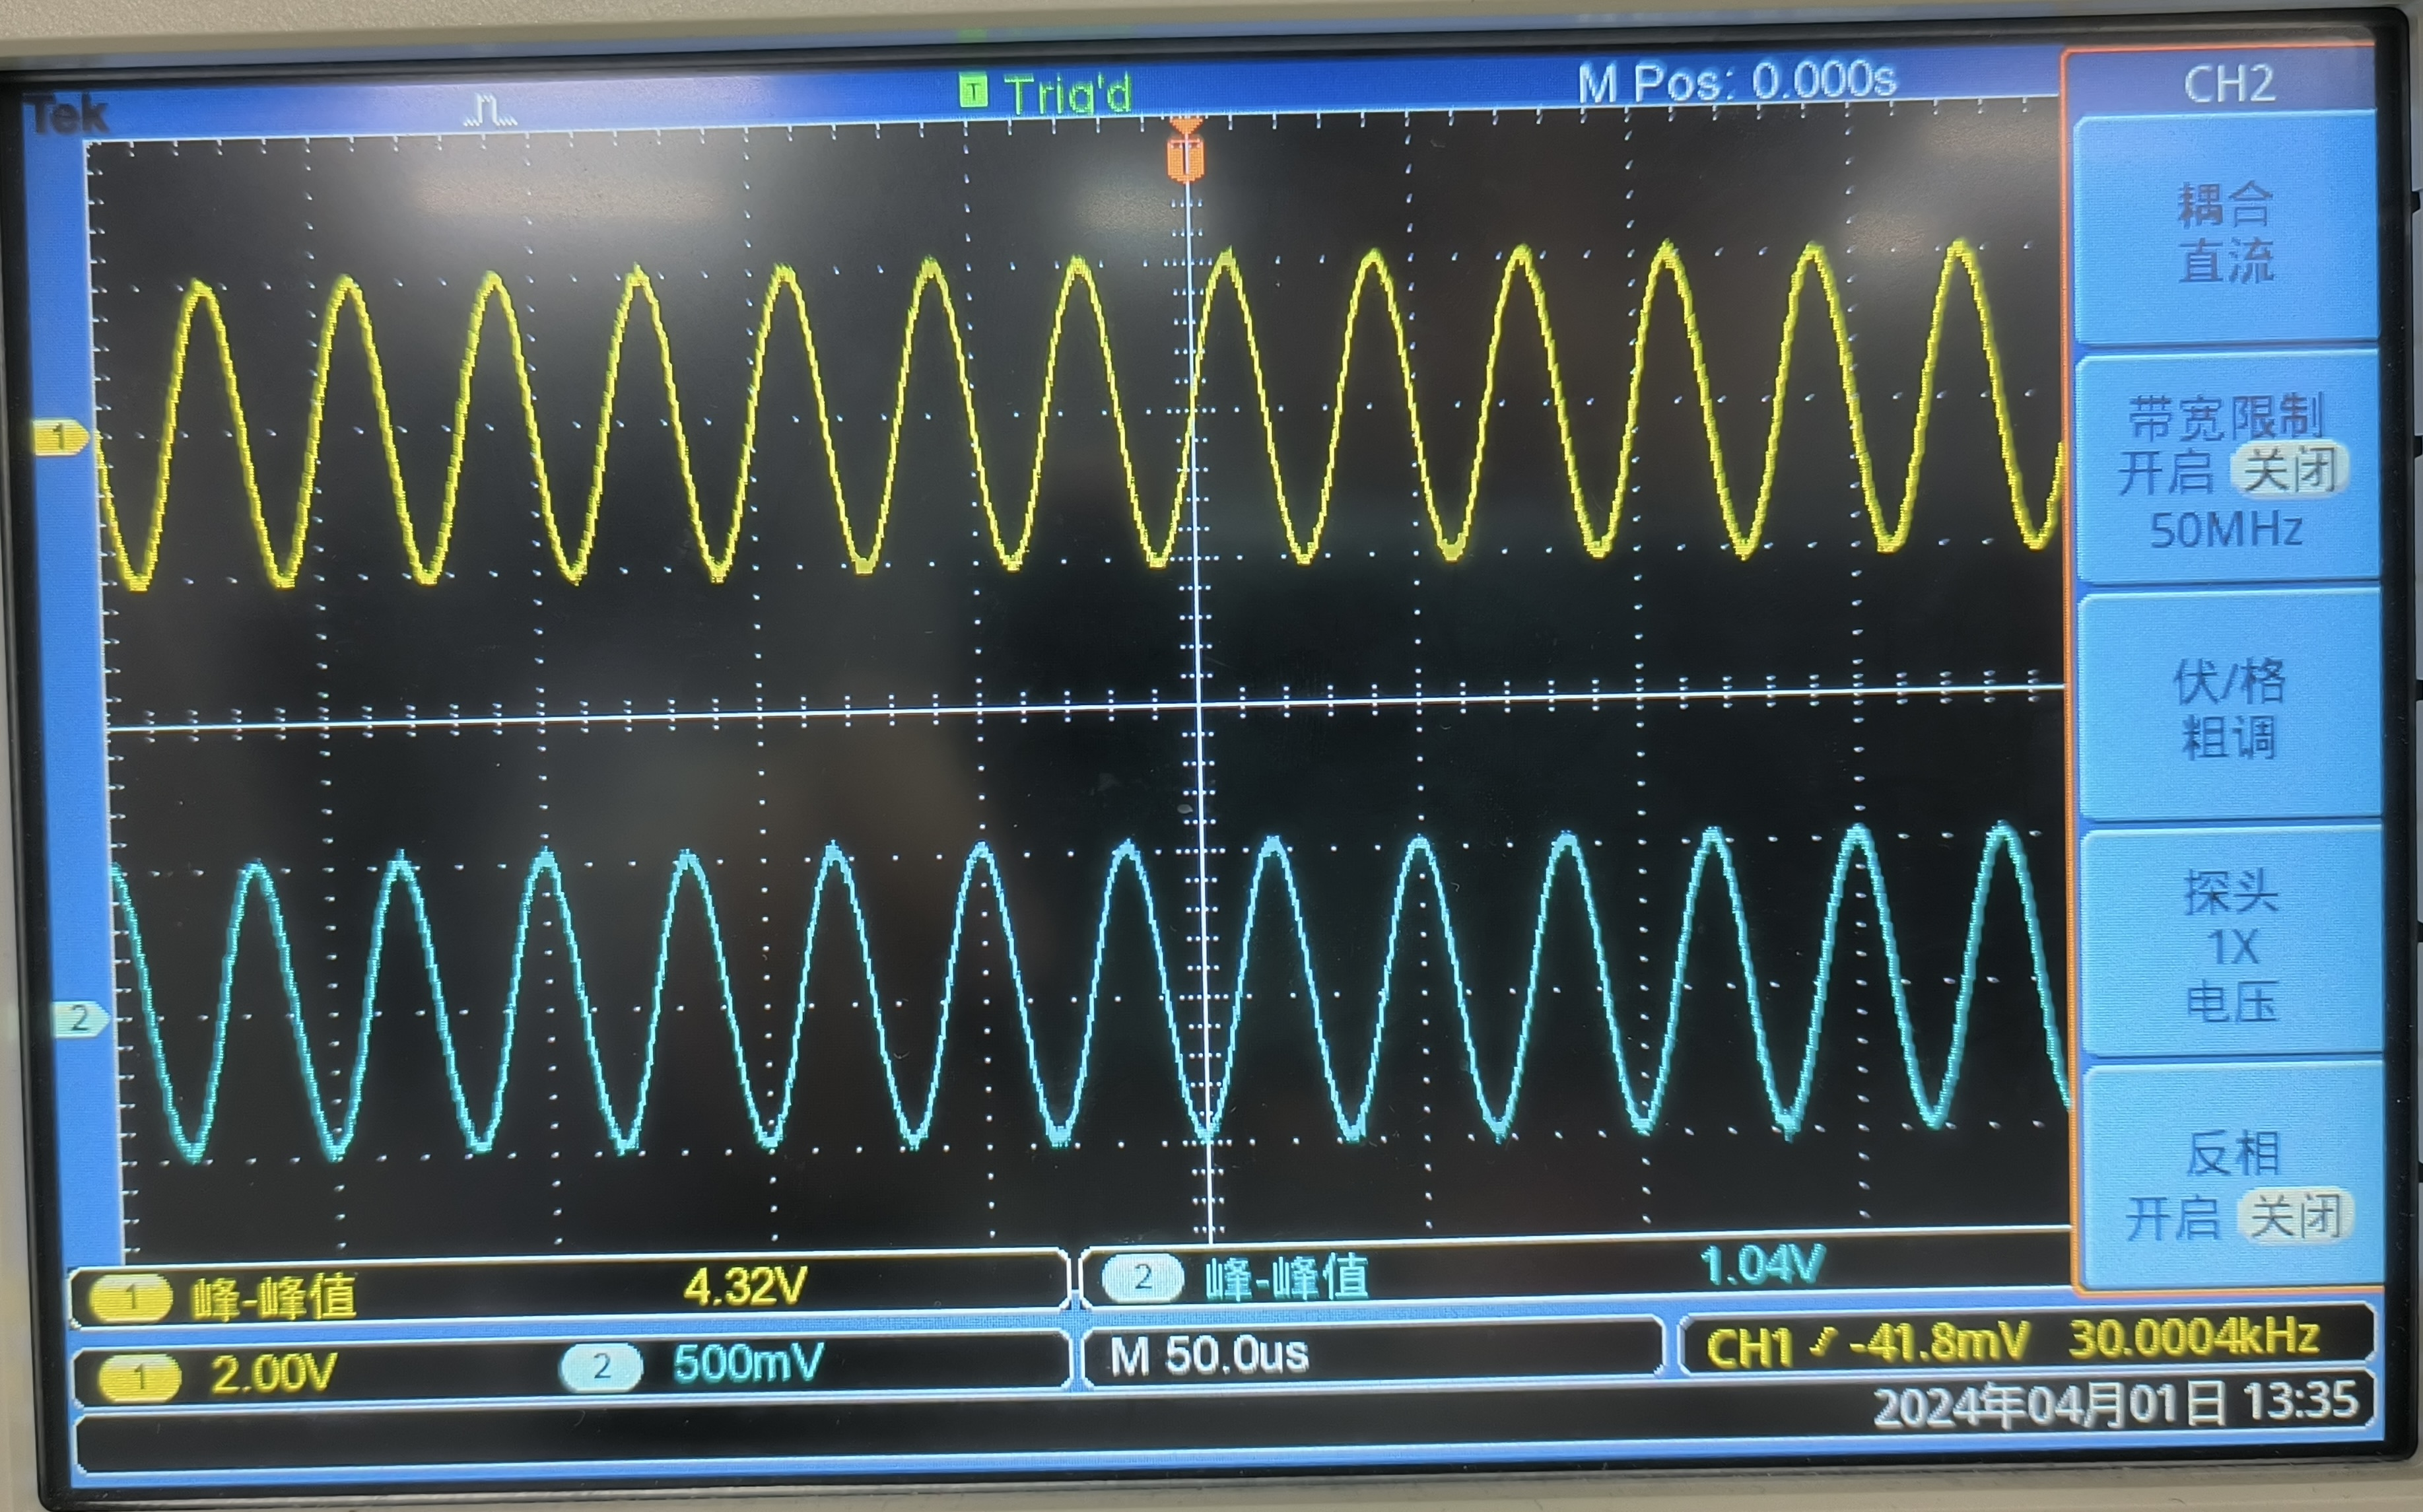
\includegraphics[width=0.6\textwidth]{30k.jpeg}
   \caption{激励信号为30kHz时波形图}
\end{figure*}

\begin{figure*}[htbp]
   \centering
   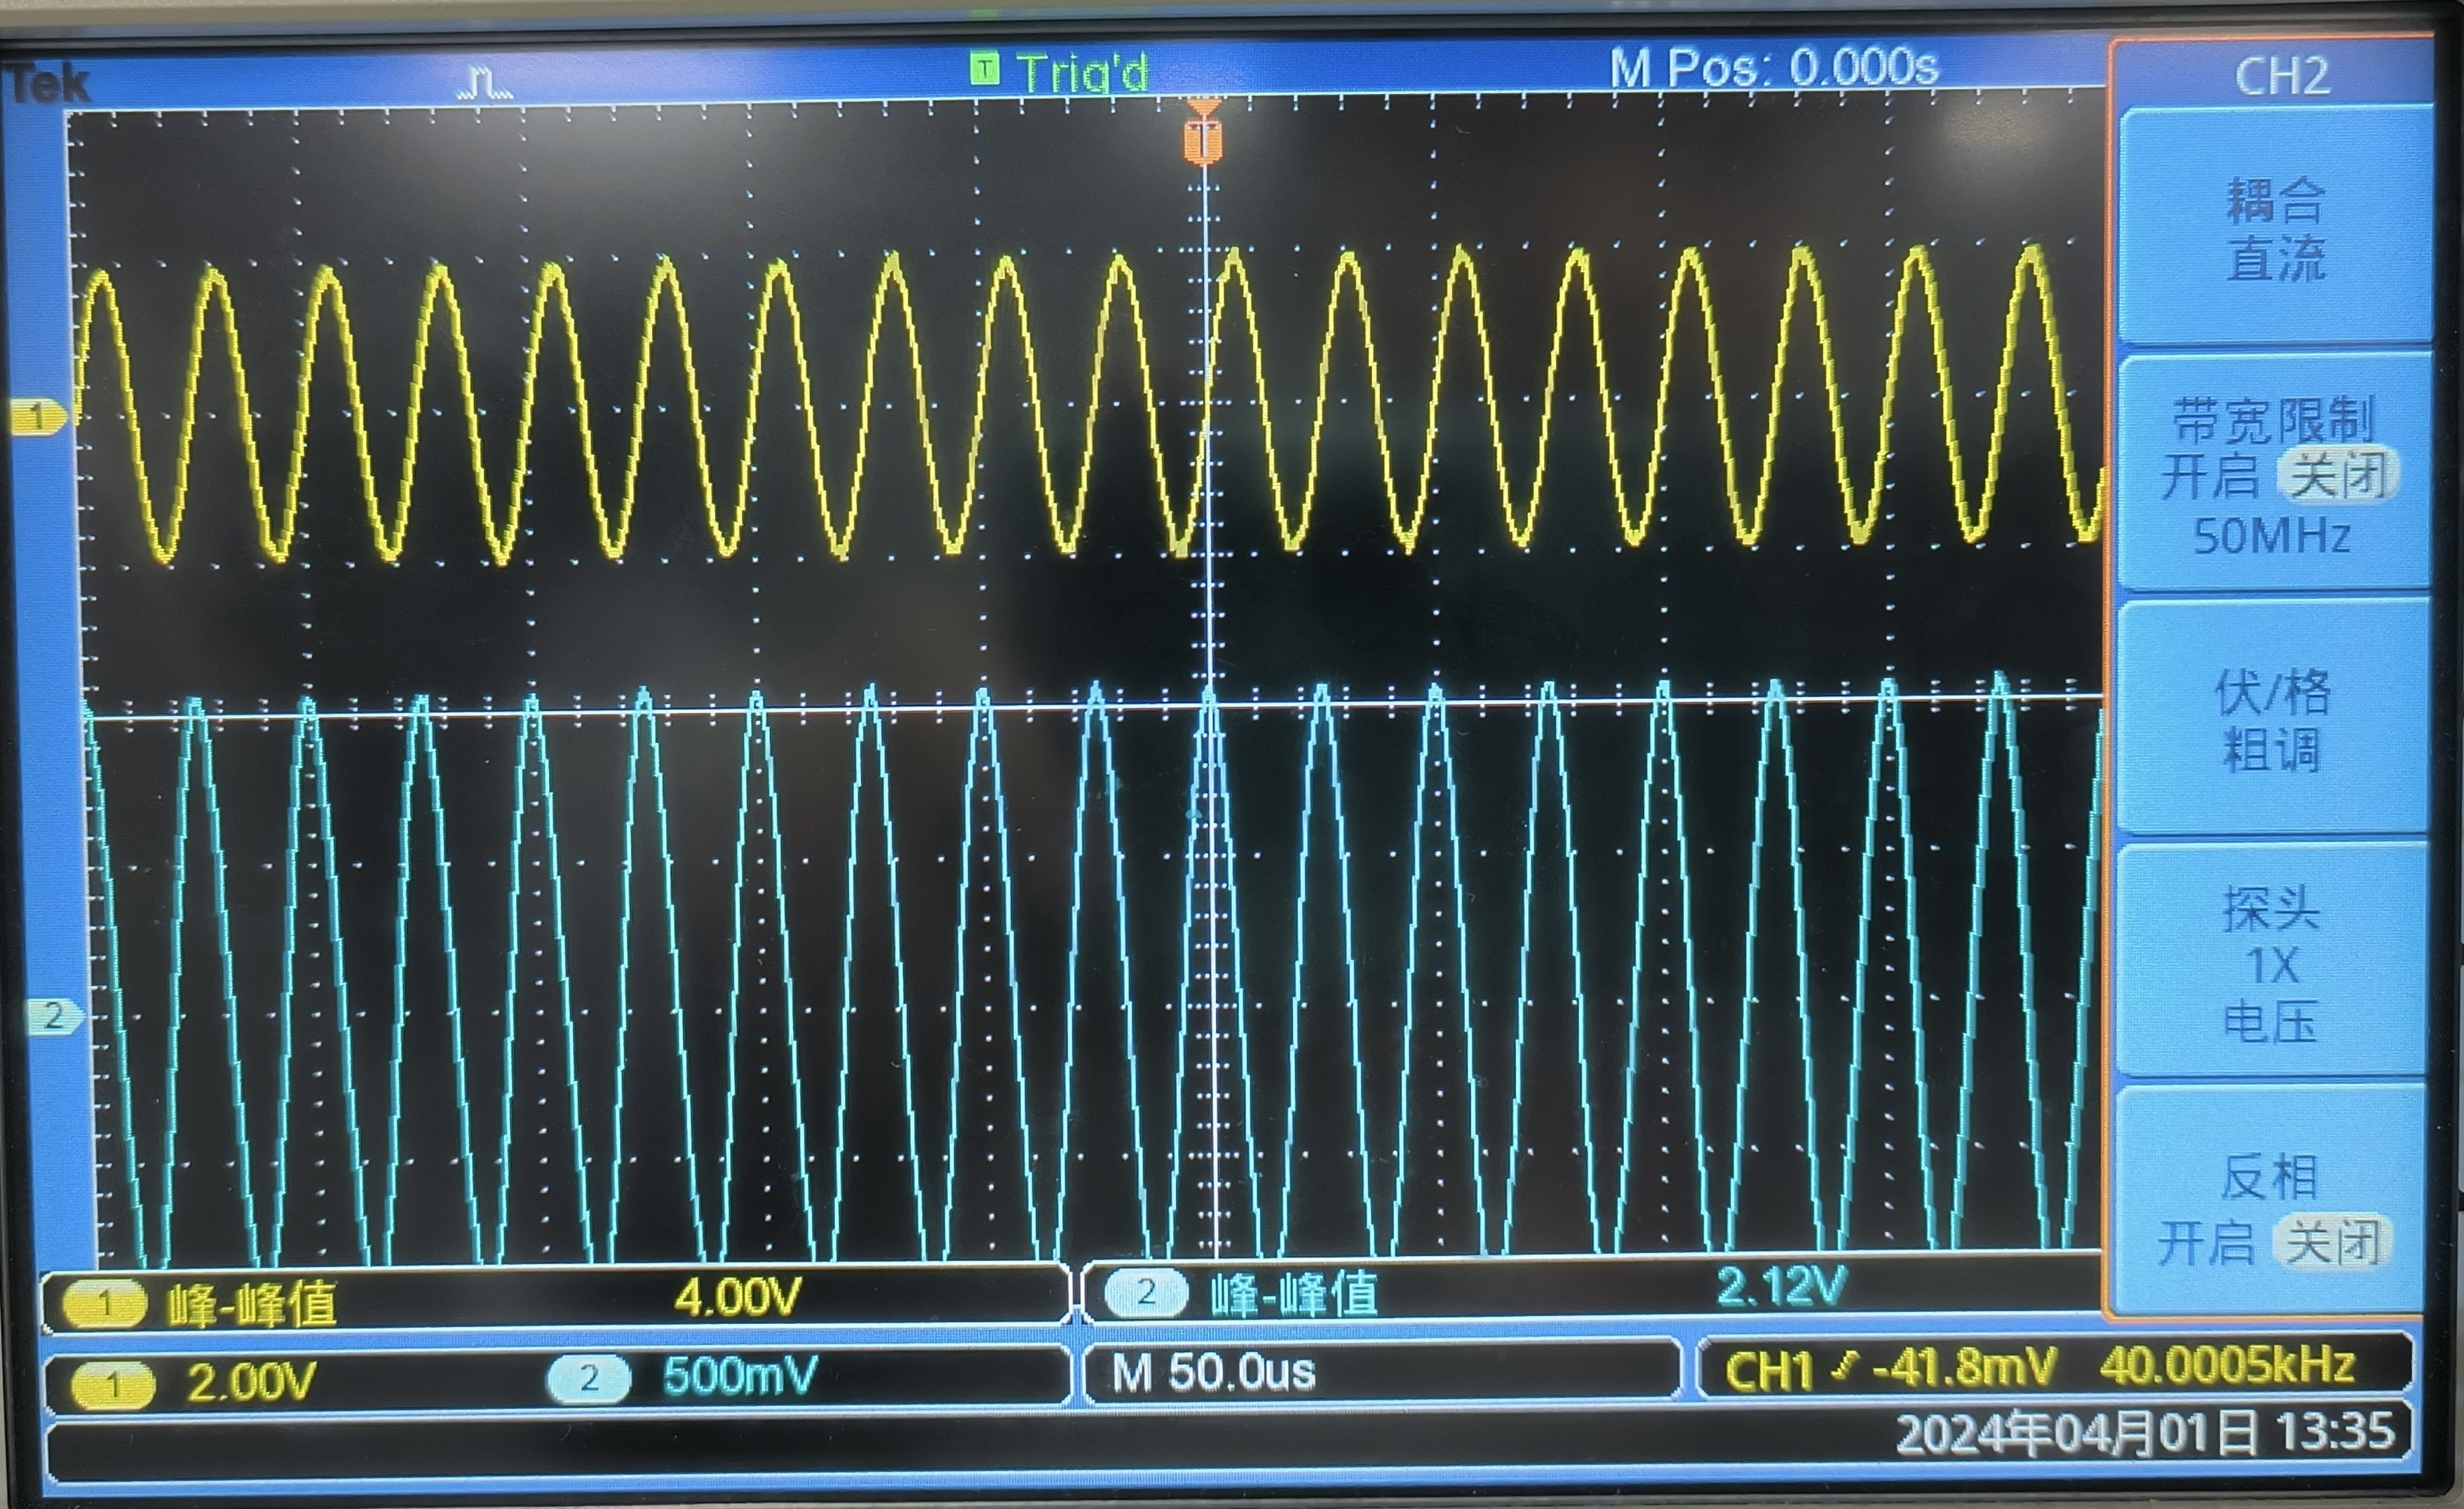
\includegraphics[width=0.6\textwidth]{40k.jpeg}
   \caption{激励信号为40kHz时波形图}
\end{figure*}

\begin{figure*}[htbp]
   \centering
   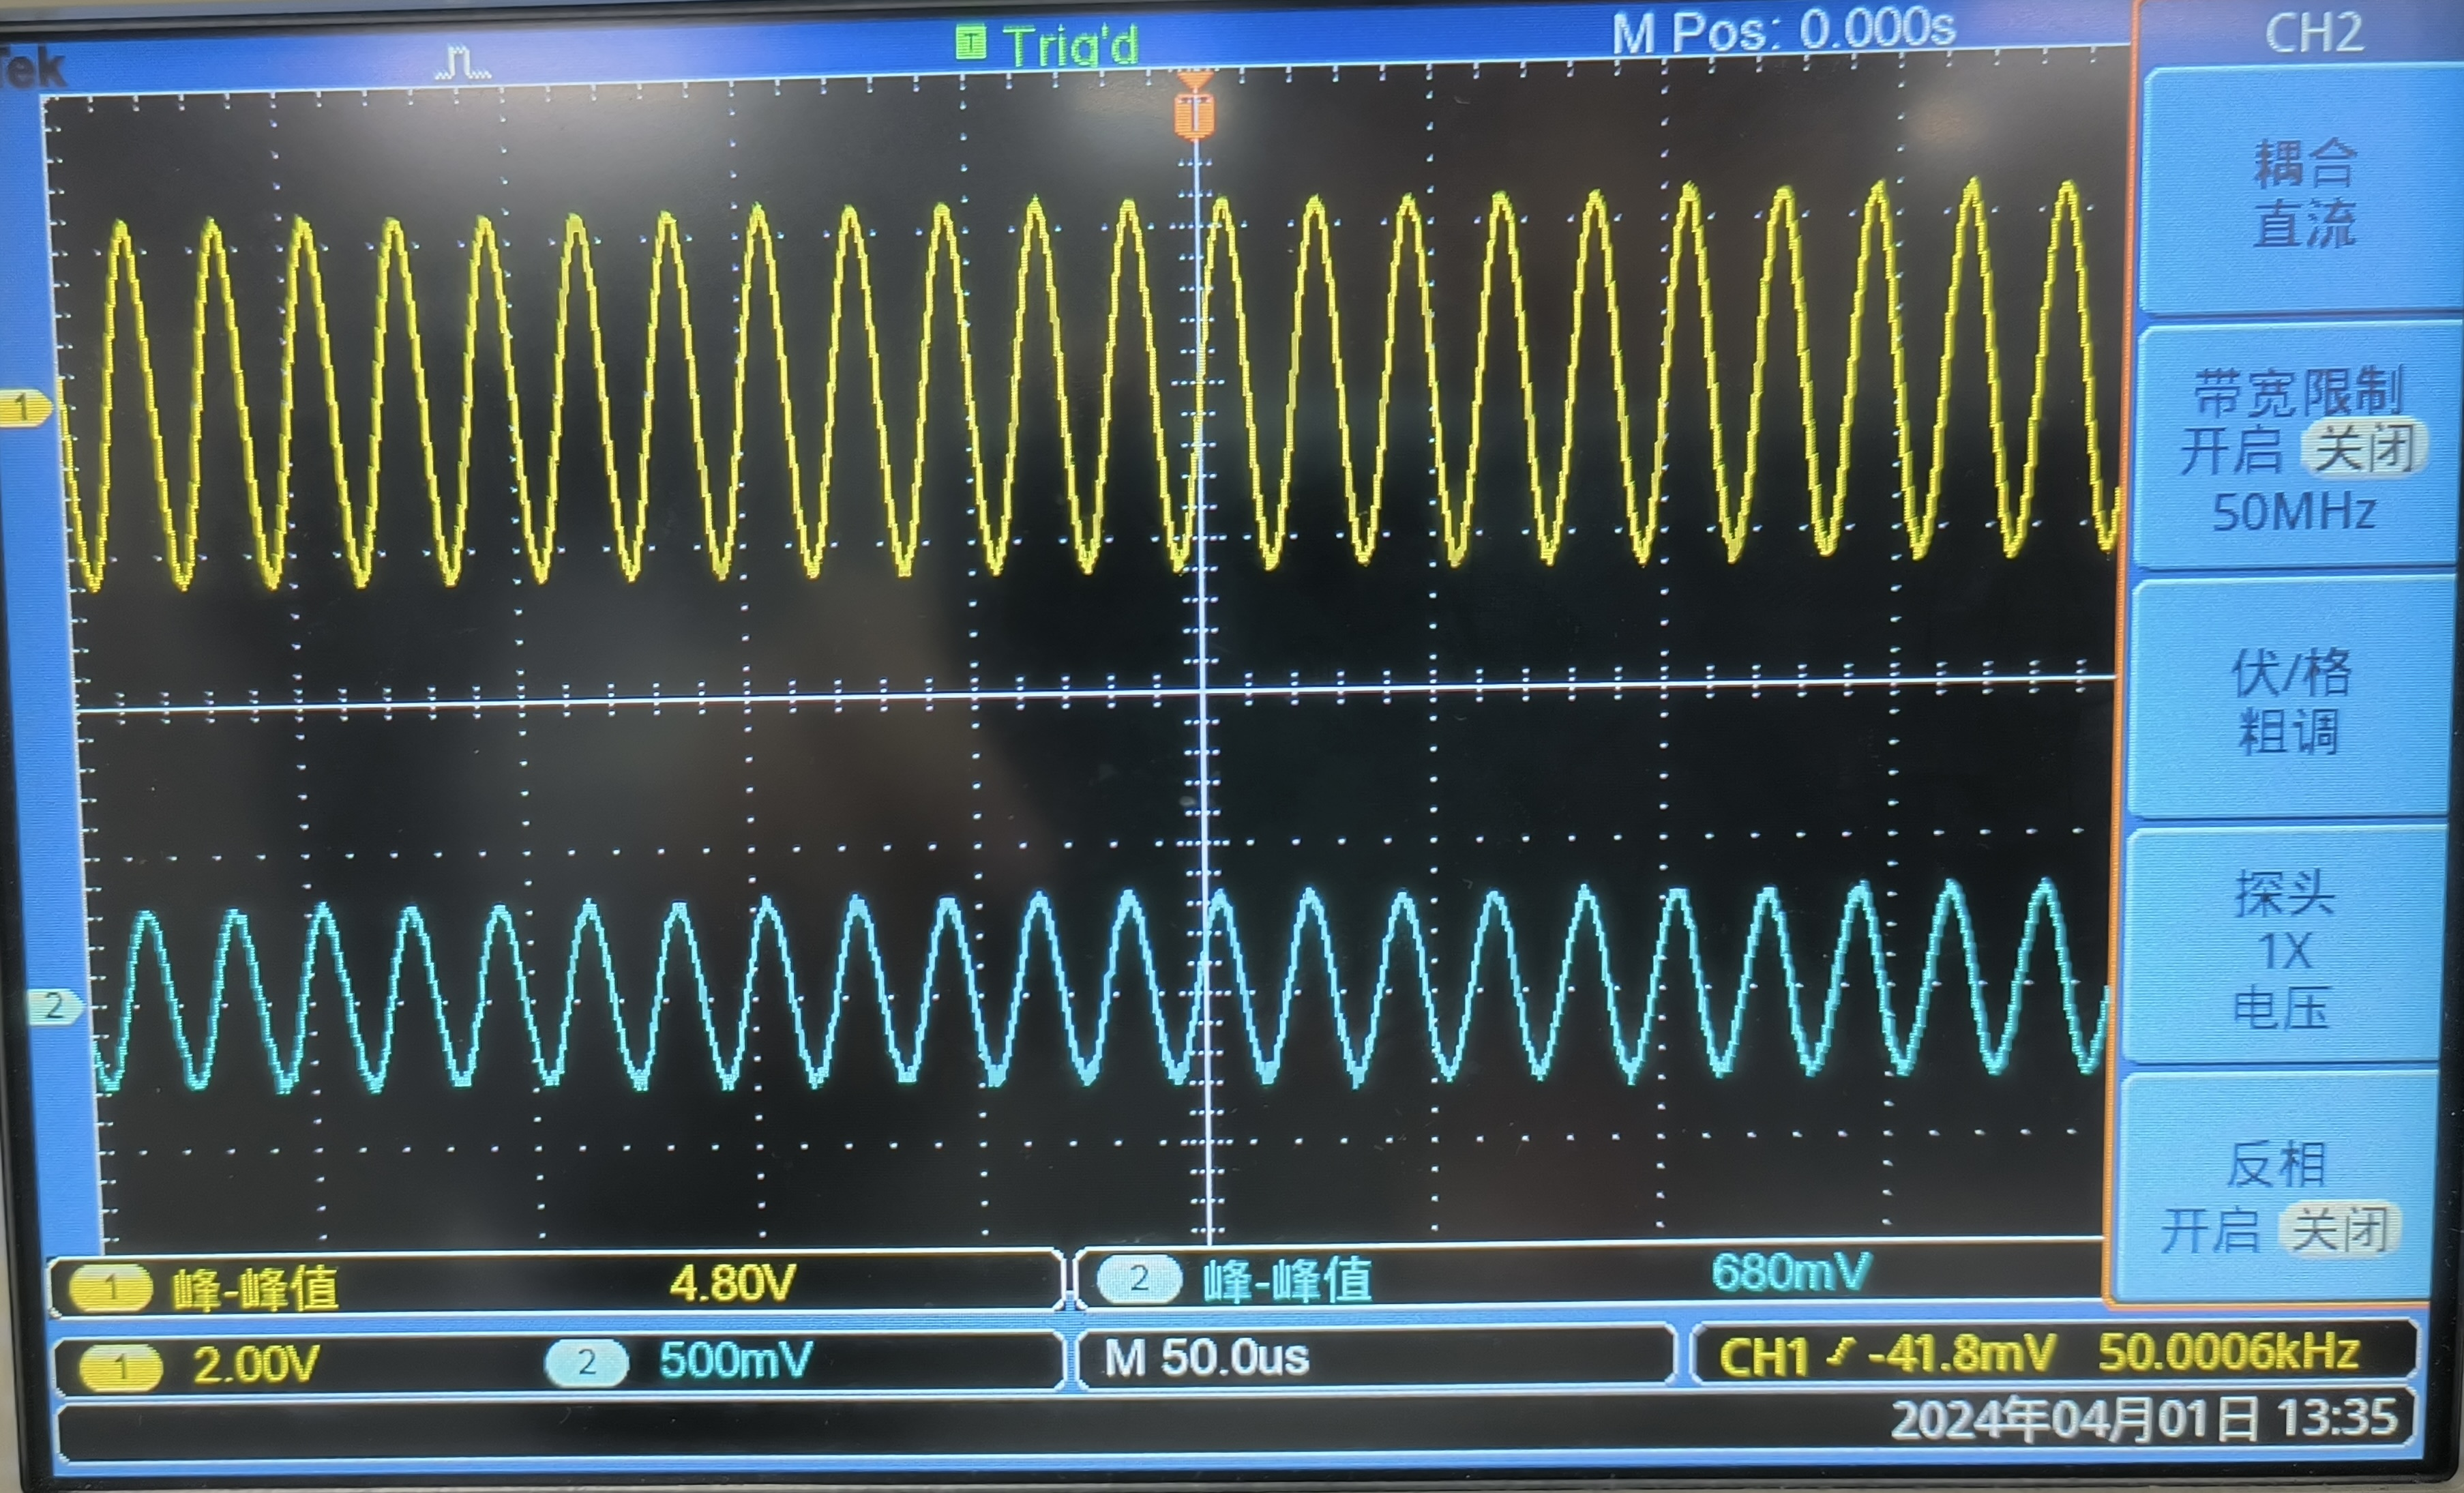
\includegraphics[width=0.6\textwidth]{50k.jpeg}
   \caption{激励信号为50kHz时波形图}
\end{figure*}

\begin{figure*}[htbp]
   \centering
   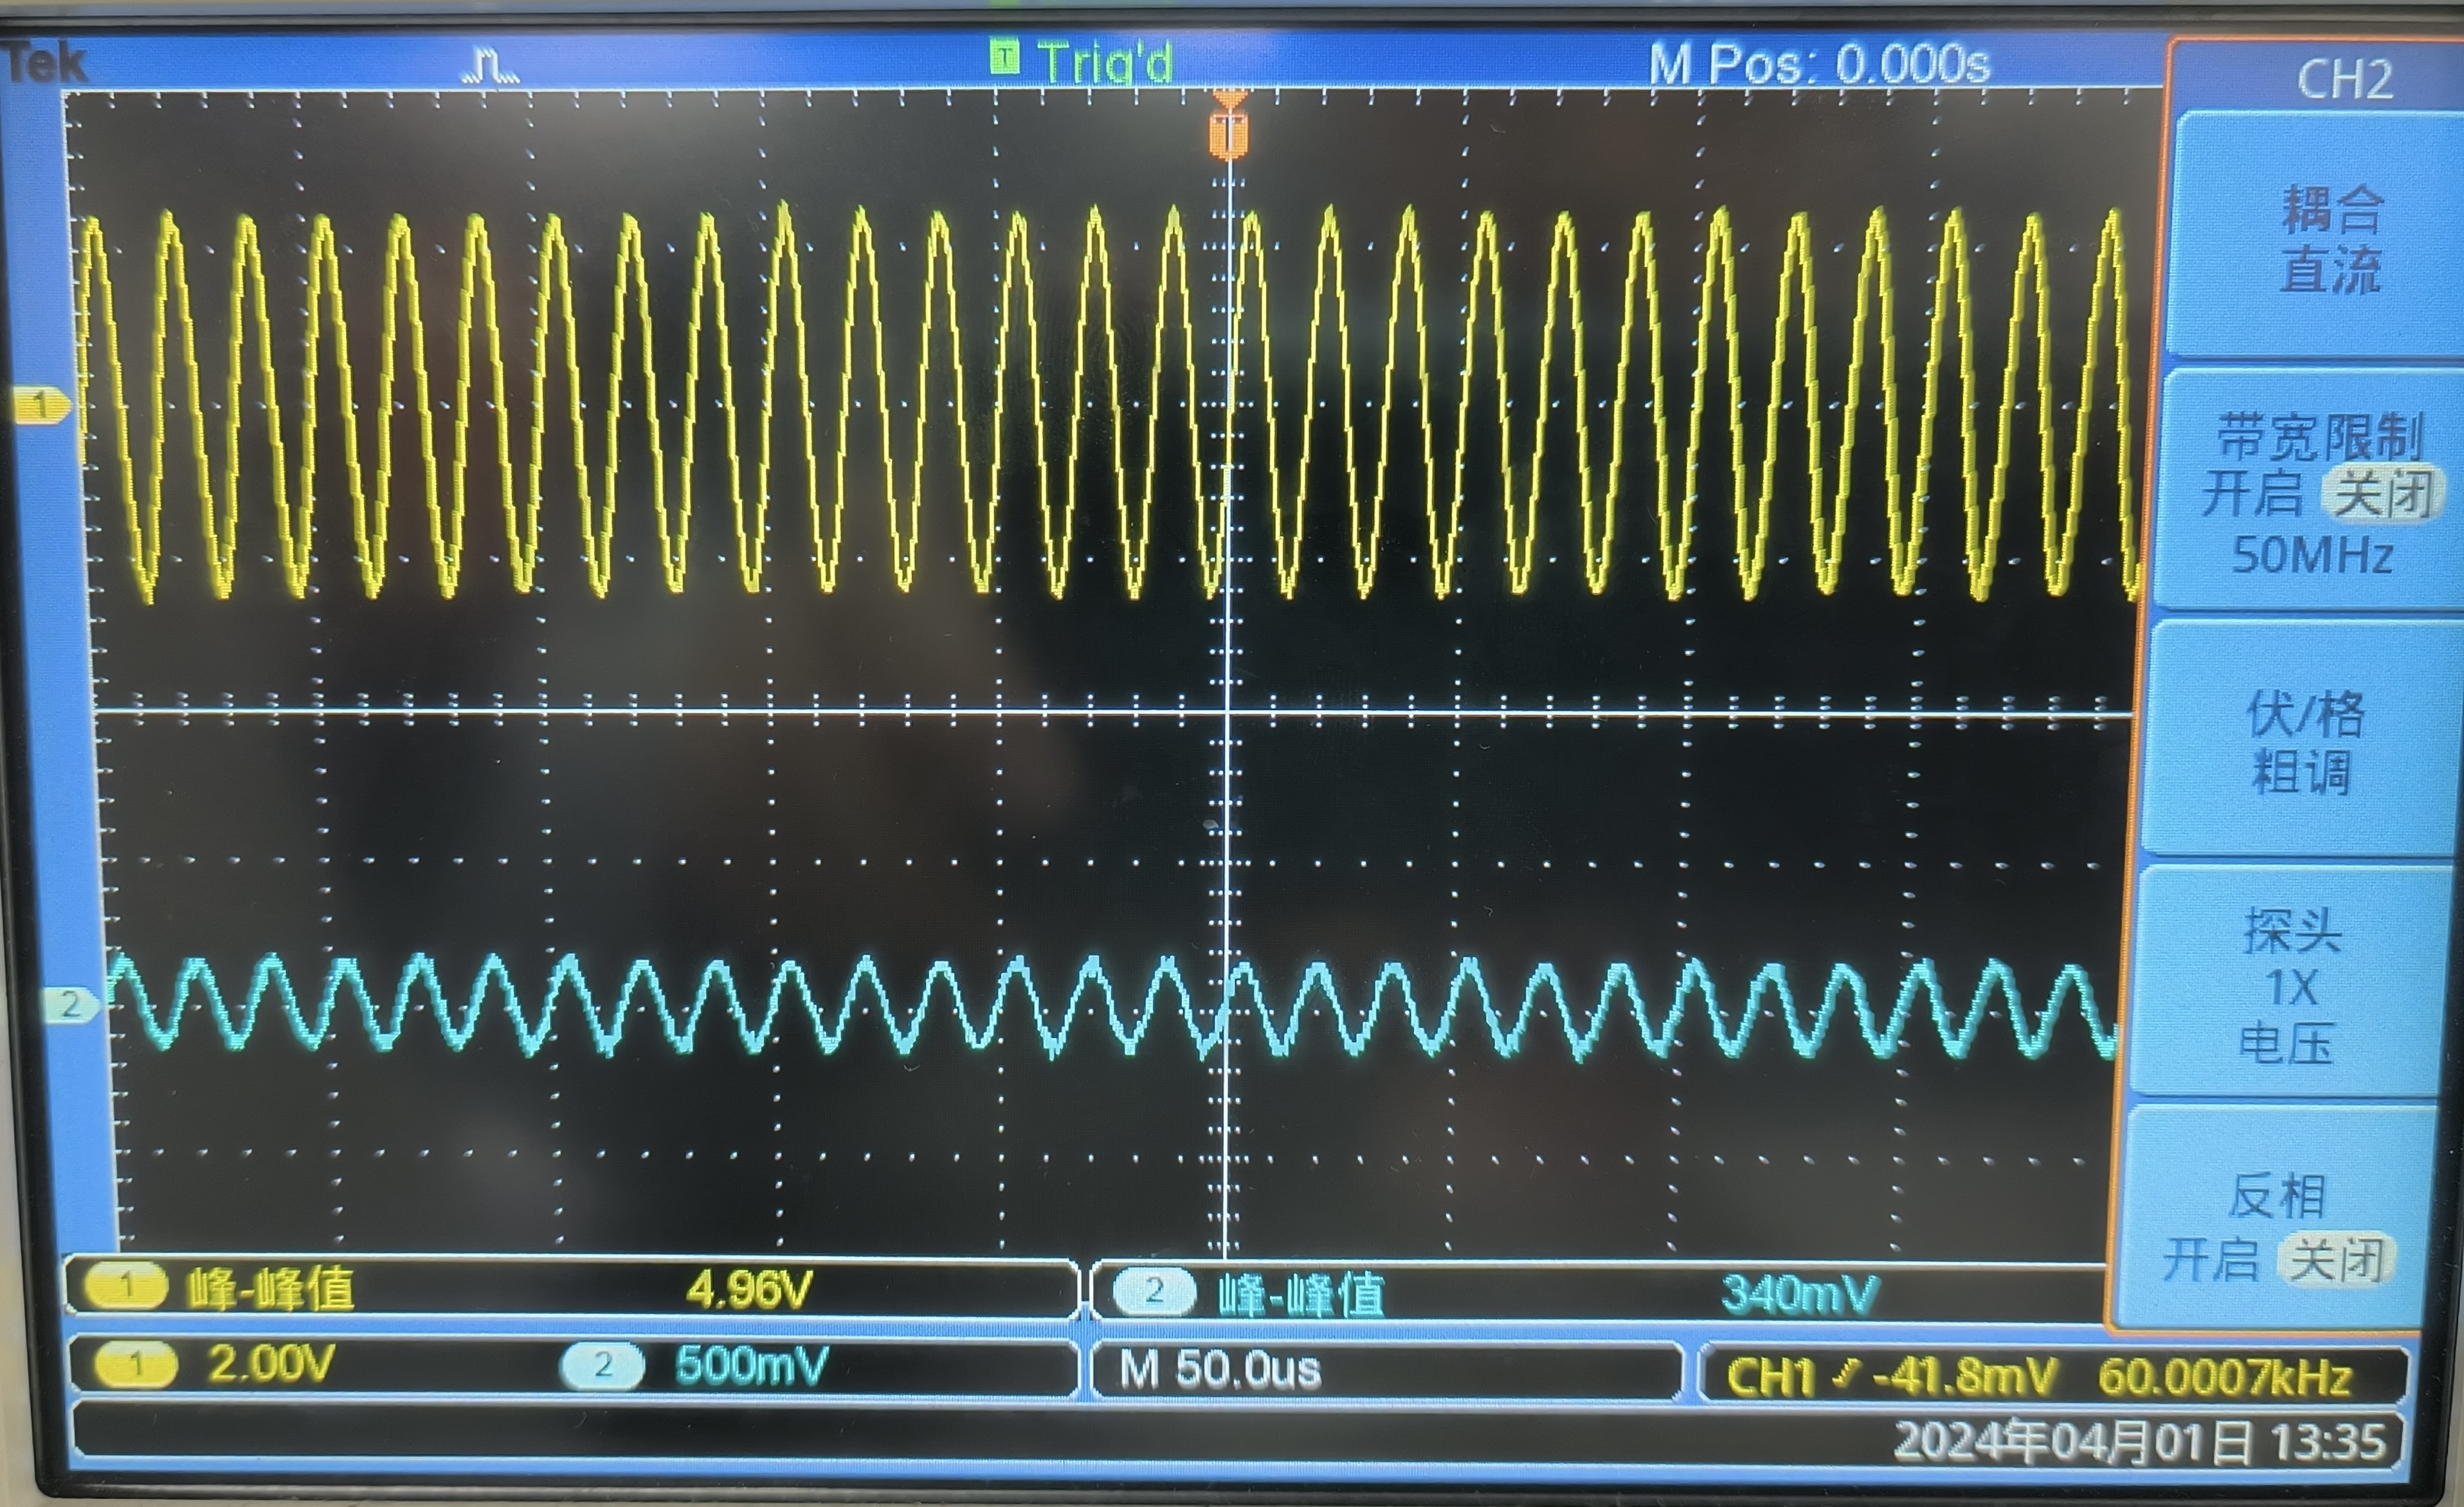
\includegraphics[width=0.6\textwidth]{60k.jpeg}
   \caption{激励信号为60kHz时波形图}
\end{figure*}

\newpage

\section{思考题}
\subsection{如何计算$\Delta x$的原点?已知线圈(含架)的宽度为$14mm$}
$\Delta x$的原点是在自感最大时的位置。所以,需要找到实验数据中$L$最大时对应的位移值,这个值即为$\Delta x$的原点。实验时,需要确保读数的刻度线位于线圈的正中央

\subsection{当激励频率升高后,零点残余电压会怎样变化?为何不能抵消?}
当激励频率升高后,零点残余电压可能会增大。

不能抵消的原因:

寄生电容的影响:电感线圈和变压器中存在寄生电容,这些寄生电容对高频信号的反应比对低频信号更为敏感。随着激励频率的增加,通过寄生电容的电流增加,导致在电路中产生更高的残余电压。

线圈电感的频率依赖性:线圈的自感量和互感量可能随频率变化。在高频条件下,线圈内部的皮肤效应和近接效应更加显著,导致有效电感量减小,这可能会影响传感器输出的零点电压。

非线性失真:传感器元件和电路可能对高频信号产生非线性响应,导致信号失真。这种失真可能会在输出中引入额外的零点偏移或残余电压。

\subsection{磁棒中的磁通是如何分布的,为什么线圈移到端部时,电感量会迅速减小?}
磁棒中的磁通分布特性主要由磁棒的材料、形状以及磁场的外部环境决定。在一个均匀的、长直磁棒内,磁通密度较为均匀分布。但在实际应用中,尤其是在电感位移传感器中,磁棒的磁通分布受到其周围环境(如线圈的位置)的显著影响。

当磁棒完全位于线圈内部时,它产生的磁场能够有效地被线圈内部的空间充满,因为磁场线倾向于在磁棒的材料内闭合,这使得线圈所环绕的磁通量最大。此时,由于线圈的自感量与其内部磁通量成正比,所以自感量达到最大值。

当线圈从磁棒的中心位置移向端部时,部分磁场线开始在磁棒外部闭合,因为磁棒的一部分不再处于线圈内部。这导致通过线圈的有效磁通量减少,因此线圈的自感量也随之减小。当线圈接近磁棒的端部时,磁场线的分布变得更加不均匀,大量磁场线在磁棒外部闭合。这是因为磁场从磁棒的一端“泄露”到空气中,形成较大的磁阻,使得穿过线圈的磁通量大幅度减少。因此,线圈的自感量在接近磁棒端部时会迅速减小。在线圈移动过程中,磁阻会随着线圈位置的变化而变化。在磁棒端部,由于磁阻突然增大,磁通量的减少更加显著。

综上所述,线圈移向磁棒端部时,电感量会迅速减小,主要是因为有效磁通量的减少以及磁阻的变化。这些效应是电感位移传感器设计和性能分析中的重要考虑因素。

\subsection{互感是如何定义的?根据本实验的仪器,设计一个测量互感的方案。}
互感定义为一个线圈电流变化率导致另一个线圈中感应电动势的量度。如果线圈1的电流变化率为\(di_1/dt\),在线圈2中产生的感应电动势为\(e_2\),则线圈1对线圈2的互感\(M_{21}\)定义为:
\[ M_{21} = \frac{e_2}{di_1/dt} \]
同样地,如果线圈2的电流变化率为\(di_2/dt\),在线圈1中产生的感应电动势为\(e_1\),则线圈2对线圈1的互感\(M_{12}\)定义为:
\[ M_{12} = \frac{e_1}{di_2/dt} \]
在理想情况下,\(M_{12} = M_{21} = M\)。

使用两个线圈,分别作为初级线圈和次级线圈。将初级线圈连接到双通道信号发生器,设置为产生正弦波信号。将次级线圈连接到双通道示波器,用于测量感应电压。通过双通道信号发生器调节激励线圈的电流,使其产生一个稳定的频率和幅度变化。使用双通道示波器观察并记录次级线圈中产生的感应电压的变化。

记录在特定电流变化率下,次级线圈中感应电压的峰值,计算互感量\(M\)。可以通过改变激励电流的变化率),并观察对应的感应电压变化,来验证互感量的一致性。可以通过调整两个线圈之间的距离和相对位置,观察互感如何随着距离和方位的变化而变化。记录不同配置下的互感值,分析线圈间距、相对方向等因素对互感的影响。

\subsection{半波整流法是如何消除零点残余电压的?优点是什么,缺点是什么?为什么说对零点判断的灵敏度很高?}
在半波整流法中,整流电路仅允许信号的一个半周期(通常是正半周期)通过,而将另一个半周期(负半周期)阻断或减至接近零。这意味着,如果输入信号包含一个小的零点偏移或残余电压,整流过程可以帮助“平均掉”这种偏移,因为它只处理信号的一部分。通过适当调整整流电路(如调整整流后的直流偏移),可以进一步减少或消除零点残余电压。

优点:
\begin{itemize}
   \item 提高零点稳定性:通过消除或减少零点残余电压,半波整流可以提高传感器输出信号的稳定性和可靠性。
   \item 简化电路设计:半波整流电路相对简单,容易实现,且成本较低。
   \item 提高灵敏度:对于零点附近的小信号变化,半波整流有助于提高系统的响应灵敏度,因为它减少了背景噪声和不必要的信号成分。
\end{itemize}

缺点:
\begin{itemize}
   \item 信号损失:由于半波整流仅利用信号的一半周期,因此可能会导致部分有用信息的损失。
   \item 效率低下:相比于全波整流,半波整流的能量利用效率较低。
   \item 可能引入畸变:整流过程可能会对信号形状产生畸变,尤其是对于非周期性或复杂信号形状。
\end{itemize}

半波整流对零点判断的高灵敏度主要是因为它通过抑制信号的一部分来减少背景噪声和非线性畸变的影响,这使得系统更容易检测和响应那些接近零点的小信号变化。此外,通过优化整流电路的设计,可以进一步提高对细微变化的响应能力,使系统对于零点附近的信号变化更为敏感。

\section{分析与讨论}
\begin{itemize}
    \item 使用示波器时,不要在一次实验中调整显示范围(scale),会影响示波器的读数
    \item 小心使用电感位移传感器,防止弄断导线连接处
    \item 改变激励信号频率需要记录多个不同频率下的波形图时,先调节至各个频率观察趋势,然后选定合适的示波器显示范围额,再进行正式实验读取电压和波形
\end{itemize}

\end{document}